\documentclass[a4paper,12 pt]{report}
\usepackage{latexsym}
\usepackage[utf8]{inputenc}



%\usepackage[english]{babel}
\usepackage[italian]{babel}

\usepackage[protrusion=true,expansion=true]{microtype}	
\usepackage{amsmath,amsfonts,amsthm} % Math packages
\usepackage[pdftex]{graphicx}	
\usepackage{mathtools}

\usepackage{hyperref}
\usepackage[table,xcdraw]{xcolor}
\usepackage{setspace}
\usepackage{amssymb}
\usepackage{listings}
\usepackage{url}

\usepackage{xcolor}
\usepackage[T1]{fontenc}
\newcommand\myworries[1]{\textcolor{red}{#1}}

\usepackage{enumitem}
\usepackage{float}
\usepackage{hyperref}
\usepackage{tikz}
\usepackage{multirow}
\usepackage{todonotes}
\usepackage{placeins}

\usepackage{graphicx}  
\usepackage{array}
\usepackage{booktabs} 
\usepackage{pifont}
\newcommand{\xmark}{\ding{55}}
\newcommand{\cmark}{\ding{51}} 

\usepackage[square,numbers]{natbib}

%per pseudocodice
\usepackage{algorithm} 
\usepackage{algorithmic}
\floatname{algorithm}{Algoritmo}
\renewcommand{\thealgorithm}{\unskip}
\newlength\myindent
\setlength\myindent{2em}
\newcommand\bindent{%
	\begingroup
	\setlength{\itemindent}{\myindent}
	\addtolength{\algorithmicindent}{\myindent}
}
\newcommand\eindent{\endgroup}
\usepackage{listings}
% package italiano
%
% Opzionale
%
%\renewcommand{\contentsname}{Sommario}
%\renewcommand{\listfigurename}{List of Figures}
%\renewcommand{\listtablename}{List of Tables}
%\renewcommand{\bibname}{Bibliografia}
%\renewcommand{\indexname}{Indice}
%\renewcommand{\figurename}{Figura}
%\renewcommand{\tablename}{Tavola}
%\renewcommand{\partname}{Parte}
%\renewcommand{\chaptername}{Capitolo}
%\renewcommand{\appendixname}{Appendice}
%\renewcommand{\abstractname}{Abstract}
%\renewcommand{\footnotesize}{\scriptsize}
%\renewcommand{\today}{\ifcase\month\or
%  Gennaio\or Febbraio\or Marzo\or Aprile\or Maggio\or Giugno\or
%  Luglio\or Agosto\or Settembre\or Ottobre\or Novembre\or Dicembre\fi
%  \space\number\day, \number\year}

% package formato
\pagestyle{plain}
\setlength{\topmargin}{0.0in}
\setlength{\headheight}{0.1in}
\setlength{\headsep}{0.0in}
\setlength{\footskip}{0.8in}
\setlength{\textheight}{9.0in}
\setlength{\textwidth}{6.0in}
\setlength{\oddsidemargin}{0.2in}
\setlength{\evensidemargin}{0.2in}
\setlength{\parindent}{0.4 in}
\onehalfspacing


\def\cent{\centerline}
\def\vs{\vskip 10 pt plus 1 pt}
\def\bs{\bf}
\def\grad{\vec{\nabla}}
\def\gradx{\vec{\nabla}_x}
\def\epsilon{\varepsilon}



\newcommand{\cvd}{\begin{flushright}$\Box$\end{flushright}}
\newcommand{\tr}{{\rm Tr}\;}
\newcommand{\eq}{\begin{equation}}
\newcommand{\feq}{\end{equation}}
\theoremstyle{definition}
\newtheorem{definition}{Definition}[section]
 
\theoremstyle{remark}
\newtheorem*{remark}{Remark}

\definecolor{blu_dmi}{HTML}{002e62}


%%%%%%%%%%%%%%%%%%%%%%%%%%%%%%%%%
%%%%%%%%%%%%%%%%%%%%%%%%%%%%%%%%%
%%%%%%%%%%%%%%%%%%%%%%%%%%%%%%%%%
%%%%%%%%%%%%%%%%%%%%%%%%%%%%%%%%%



\begin{document}
    % Thesis frontmatter --------------------------------------------

\thispagestyle{empty} %suppress page number

	\noindent % just to prevent indentation narrowing the line width for this line
	
\includegraphics[width=0.15\textwidth]{img/logoUniPg}
	\begin{minipage}[b]{0.7\textwidth}
		\centering
		{\Large{\textsc{Universit{\`a} di Perugia}}}\\
		\vspace{0.4 em}
		{\large {Dipartimento di Matematica e Informatica}}
		\vspace{0.6 em}
	\end{minipage}%
	
\includegraphics[width=0.15\textwidth]{img/logoDMI}
	
	\vspace{8 em}

	\begin{center}
		

	
		{\Huge{Appunti Knowledge Representation and Automated Reasoning }}\\
		\vspace{2 em}
		{\large { Autore: Chiara Luchini}}\\
		\vspace{5 em}
		{\large {Basati su:}}\\
		{\large {- Slides del Prof. Stefano Bistarelli}}\\
		{\large {- Lezioni del Prof. Stefano Bistarelli}}\\
		%{\large \textcolor{blu_dmi}{- Appunti lezioni online Prof. Alfredo Navarra}}\\
		
	
	

%		\makebox[380pt][c]{\textcolor{blu_dmi}{\textit{Advisor} \hfill \textit{}}}
%		\makebox[380pt][c]{\textcolor{blu_dmi}{\textbf{Dott. Francesco Santini \hfill}}}
		
		\vspace{6 em}
		\vfill
		
	{\rule{380pt}{.4pt}}\\
		\vspace{1.2 em}
		\large{{Anno Accademico 2021/2022}}
		
		
		
		
	\end{center}

% ------------------------------------------------------------------
    \newpage
  	\tableofcontents
    \newpage
    %\lstlistoflistings
	\newpage
	\listoffigures
    \newpage
    \chapter{Costraint Satisfaction Problems}
\subsection{Constraint Satisfaction}
Un vincolo è semplicemente una relazione logica tra diverse incognite (o variabili), ognuna delle quali assume un valore in un dato dominio. Un vincolo quindi restringe i possibili valori che le variabili possono assumere ne rappresenta alcune informazioni parziali sulle variabili di interesse. Formalmente, un costraint satisfaction problem (o CSP) è definito da:
\begin{itemize}
    \item Un insieme di \textbf{variabili} $X1, X2, \cdots , X_n$;
    \item Una funzione che mappa ogni variabile a un dominio finito;
    \item Un insieme di \textbf{vincoli} $C1, C2, \cdots, C_m$;
    \item Un insieme $D_i$ non vuoto di possibili valori per ogni variabile $X_i$.
\end{itemize}  
 Ogni vincolo $C_i$ coinvolge alcuni sottoinsiemi di variabili e specifica le combinazioni di valori consentite per quel sottoinsieme. Uno \textbf{stato} del problema è definito da un'\textbf{assegnazione di valori} ad alcune o a tutte le variabili $\{ X_i = v_i, X_j = v_j, \cdots\}$. Un'assegnazione che non viola alcun vincolo è chiamata assegnazione \textbf{coerente o legale}. Un'\textbf{assegnazione completa} è quella in cui viene menzionata ogni variabile, e una \textbf{soluzione} a un CSP è un'assegnazione completa che soddisfa tutti i vincoli. Alcuni CSP richiedono anche una soluzione che massimizzi una \textbf{funzione obiettivo}. Ciascun vincolo limita la combinazione di valori che un insieme di variabili può assumere contemporaneamente. Una soluzione di un CSP è l'assegnazione a ciascuna variabile di un valore dal suo dominio che soddisfi tutti i vincoli. Il compito è trovare una soluzione o tutte le soluzioni. Pertanto, il CSP è un problema combinatorio che può essere risolto mediante la ricerca.
\subsection{Constraint Solving} 
La risoluzione dei vincoli differisce dalla soddisfazione dei vincoli poiché utilizza variabili con domini infiniti come i numeri reali. Inoltre, i singoli vincoli sono più complicati, ad esempio non lineari, uguaglianze...
\subsection{Esempio: Map-Colouring} 
Lavoriamo in una mappa dell'Australia che mostra ciascuno dei suoi stati e territori e il compito ci viene affidato è di colorare ogni regione di rosso, verde o blu in modo tale che le regioni vicine non hanno lo stesso colore. Per formulare questo come un CSP, definiamo le variabili come le regioni: WA, NT, Q, NSW , V , SA e T. Il dominio di ciascuna variabile è l'insieme $\{rosso, verde, blu\}$. I vincoli richiedono che le regioni vicine abbiano colori distinti; ad esempio, le combinazioni consentite per WA e NT sono le coppie 
\[\{(rosso, verde),(rosso, blu),(verde, rosso),(verde, blu),(blu, rosso),(blu, verde)\}\]
Ci sono molte soluzioni possibili, come  $\{WA = rosso, AND = verde, A = rosso, NSW = verde, V = rosso, SA = blu, T = rosso\}$.

È utile visualizzare un CSP come \textbf{grafico di vincoli}. I nodi
del grafico corrispondono a variabili del problema e gli archi corrispondono a vincoli.
\begin{figure}[H]
	\centering
    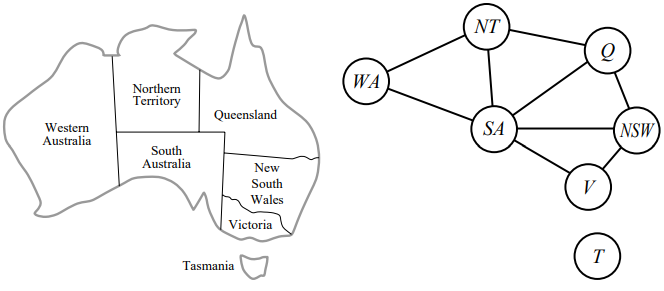
\includegraphics[width=15cm, keepaspectratio]{img/map_colouring.png}
	\caption{Map-colouring}\label{fig:map_colouring}
\end{figure}
\begin{figure}[H]
	\centering
    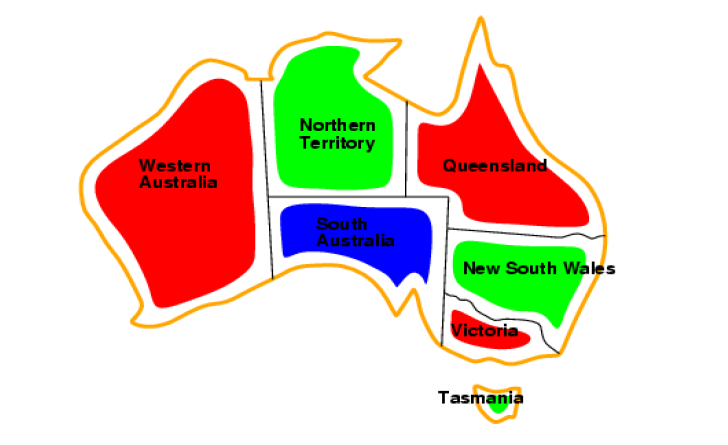
\includegraphics[width=14cm, keepaspectratio]{img/sol_map_coulouring.png}
	\caption{Soluzione Map-colouring}\label{fig:sol_map_colouring}
\end{figure}
In un CSP binario ogni vincolo è in relazione con due variabile. Il tipo più semplice di CSP coinvolge variabili che sono discrete e hanno domini finiti, i problemi di colorazione della mappa sono di questo tipo.
\paragraph{Tipi di variabili.} Le variabili discrete possono avere domini:
\begin{itemize}
    \item \textbf{finiti}: grandezza dell'assegnamento completo $d \longrightarrow O(d^n)$;
    \item \textbf{infiniti}: \begin{itemize}
        \item hanno bisogno di un linguaggio di vincoli
        \item i vincoli lineari sono risolvibili, i non lineari sono indecidibili;
    \end{itemize}
\end{itemize}
Le variabili continue con dei vincoli lineari sono risolvibili in un tempo polinomiale dai metodi LP. 

\paragraph{Tipi di vincoli.} I vincoli possono essere:
\begin{itemize}
    \item \textbf{unari}: coinvolgono una sola variabile;
    \item \textbf{binari}: coinvolgono due variabili;
    \item \textbf{higher-order}: coinvolgono 3 o più variabili;
    \item \textbf{preferenze}: es. \textit{il rosso è meglio del verde}, spesso rappresentabili come un costo associato a ogni assegnamento di variabile.
\end{itemize}
Inoltre i vincoli possono essere espressi in maniera:
\begin{itemize}
    \item \textbf{Implicita}: non viene direttamente indicata la relazione fra gli elementi del dominio che sono permessi. Un esempio può essere x<y, dove non si elencano tutti i possibili assegnamenti delle variabili che non violano quel vincolo ma si possono calcolare;
    \item \textbf{Esplicita}: si elencano tutti i valori ammessi per le variabili coinvolte nel vincolo. Nell'esempio di prima si avranno tutte le coppie di valori ammessi in base a quel vincolo.
\end{itemize}
\subsection{Caratteristiche CSP}
Alcune caratteristiche di questi problemi sono:
\begin{itemize}
    \item Caso speciale di un problema di ricerca;
    \item I domini possono essere discreti o continui;
    \item Commutatività: l'ordine in cui applichiamo le azioni non ha effetto: ad ogni nodo, considera solo le assegnazioni ad una singola variabile;
    \item Durante la ricerca, una volta violato un vincolo, rimane tale (monotonicità): fermati e torna indietro non appena un vincolo viene violato;
    \item L'ordine in cui scegliamo le variabili e i loro valori fa una grande differenza: abbiamo bisogno di un'euristica intelligente;
    \item Il test dell'obiettivo è scomposto in un insieme di vincoli sulle variabili, piuttosto che in una singola scatola nera;
    \item Quando gli insiemi di variabili sono indipendenti (nessun vincolo tra di loro) il problema è scomponibile in sottoproblemi che possono essere risolti indipendentemente;
    \item A ogni passaggio dobbiamo verificare la coerenza. Abbiamo bisogno di metodi di propagazione dei vincoli.
\end{itemize}

\subsection{Standard search formulation }
Gli stati sono definiti dal valore assegnato finora:
\begin{itemize}
    \item \textbf{Stato iniziale}: assegnamento vuoto \{\};
    \item \textbf{Funzione successore}: assegna un valore a una variabile non assegnata che non va in conflitto con l'assegnamento corrente;
    \item \textbf{Goal test}: l'assegnamento corrente è completo.
\end{itemize}
Questa formula viene usata per tutti i CSP e ogni soluzione appare a profondità n con n variabili. Il cammino è irrilevante, così che può usare la formulazione complete-state.


\section{Metodi di ricerca sistematici}
\subsection{Generate \& test}
Probabilmente il metodo di risoluzione dei problemi più generale. L'algoritmo consiste nei seguenti due passaggi che si ripetono:
\begin{enumerate}
    \item si generano le etichette;
    \item si controlla se vanno bene gli assegnamenti.
\end{enumerate}
Alcuni possibili miglioramenti sono ad esempio uno \textbf{smart generator}, ovvero si assegnano i valori alle variabili e se non vanno bene si effettuano dei cambiamenti sugli assegnamenti errati (ricerca locale). Un altro miglioramento consiste nel fare il test sugli assegnamenti e poi fare backtracking. 
\subsection{Backtraking}
Supponiamo di avere un problema CSP con 4 variabili (A,B,C,D), supponiamo che i vincoli siano 
\[A=D, B \neq D, A+C < 4\]
L'algoritmo consiste in:
\begin{enumerate}
    \item assegna il valore alla variabile;
    \item si controlla la consistenza;
    \item finché tutte le variabili sono etichettate.
\end{enumerate}

\begin{figure}[H]
	\centering
    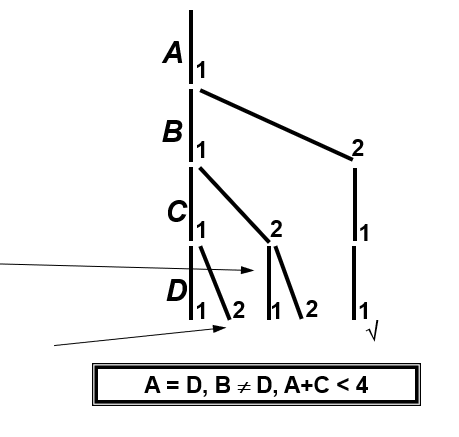
\includegraphics[width=7cm, keepaspectratio]{img/backtrack.png}
	\caption{Esempio backtracking.}\label{fig:es_backtracking}
\end{figure}
\noindent Se tutte le variabili non sono etichettate si torna al passo 1. 
 L'assegnamento delle variabili è commutativo ad esempio 
\begin{center}
  [WA = red allora NT = green] come [NT=green allora WA =red]  
\end{center}

\noindent Si devono solo considerare gli assegnamenti alle singole variabili per ogni nodo $\longrightarrow b = d $ e ci sono $d^n$ foglie.
La \textbf{DFS} per i CSP son gli assegnamenti a variabili singole è chiamata ricerca \textbf{backtracking}, essa è l'algoritmo base uniformed per i CSP.

\begin{figure}[H]
	\centering
    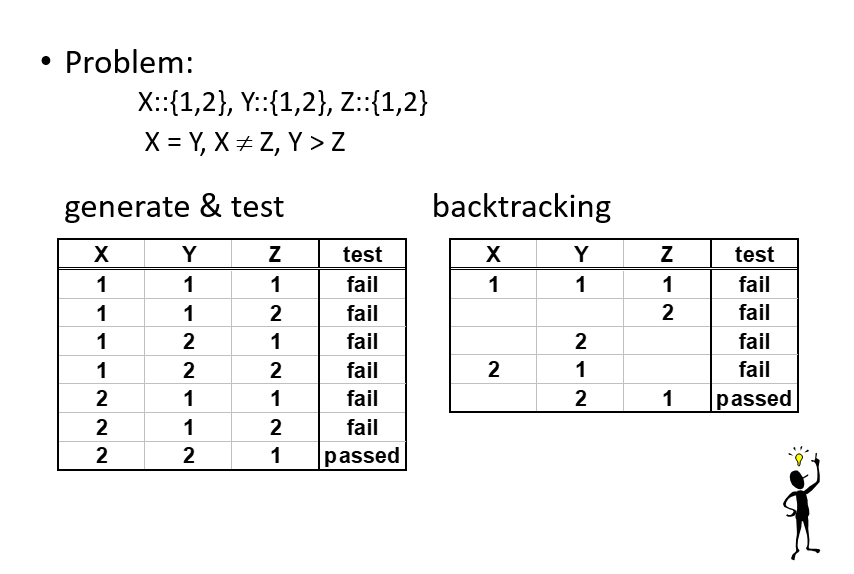
\includegraphics[width=13.5cm, keepaspectratio]{img/diff_generate_backtracking.png}
	\caption{Esempio generate and test vs backtracking.}\label{fig:diff_generate_backtracking}
\end{figure}

\subsubsection{Ricerca backtracking: incrementale}
La strategia di ricerca è la\textbf{ DFS (Depth First Search):}
\begin{enumerate}
    \item scegli una variabile non istanziata, scegli un valore dal suo dominio, controlla se qualche vincolo è violato;
    \item se nessun vincolo viene violato, continua la ricerca in modo ricorsivo;
    \item altrimenti, torna indietro: torna alla decisione precedente e fai un'altra scelta.
\end{enumerate}
In termini di grandezza dell'albero di ricerca il numero di foglie è pari a $d^n$, dove n è il numero di variabili e d = $max|D_i|$.
\begin{figure}[H]
	\centering
    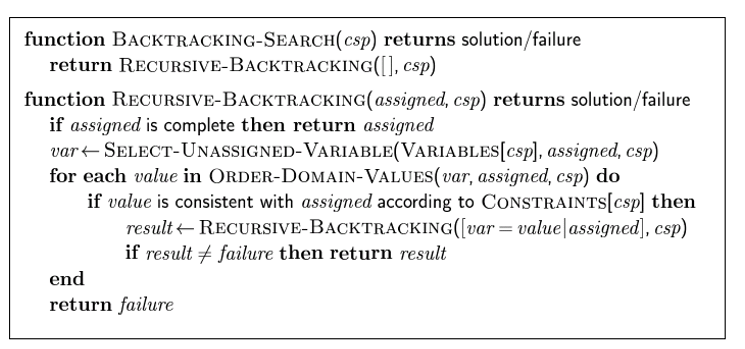
\includegraphics[width=14cm, keepaspectratio]{img/alg_backtracking.png}
	\caption{Algoritmo di backtracking.}\label{fig:alg_backtracking}
\end{figure}

\begin{figure}[H]
	\centering
    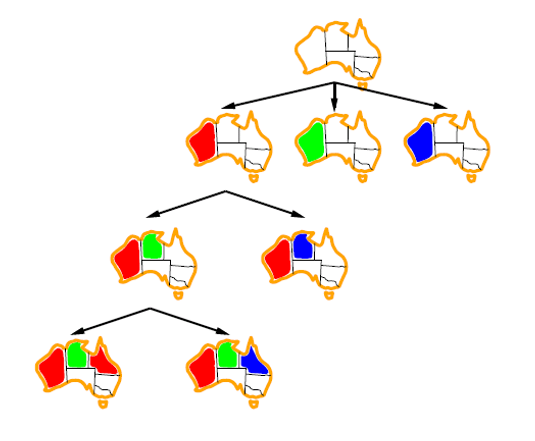
\includegraphics[width=10cm, keepaspectratio]{img/es_backtracking.png}
	\caption{Esempio backtracking.}\label{fig:es_backtracking}
\end{figure}

\subsection{Miglioramenti dell'efficienza del backtracking}
Per impostazione predefinita, SELECT-UNASSIGNED-VARIABLE seleziona semplicemente la successiva variabile non assegnata nell'ordine dato dalla lista VARIABLES[csp]. Questo ordinamento di variabili statiche raramente si traduce nella ricerca più efficiente. Ad esempio, dopo le assegnazioni per WA = rosso e NT = verde, c'è un solo valore possibile per SA, quindi ha senso assegnare SA = blue next piuttosto che assegnare Q. Infatti, dopo l'assegnazione di SA, le scelte per Q, NSW e V sono tutte forzate.
\paragraph{Variabile più vincolata} In questo caso si va a scegliere fra le variabili disponibili per l'assegnamento quella più vincolata in base ad alcune caratteristiche:
\begin{itemize}
    \item si sceglie la variabile con il \textbf{minor numero di valori legali} (minimum remaining values -MRV). È stata anche chiamata la "variabile più vincolata" o euristica "fail-first", quest'ultima perché seleziona una variabile che ha maggiori probabilità di causare un errore presto, potando così l'albero di ricerca.
    \begin{figure}[H]
    	\centering
        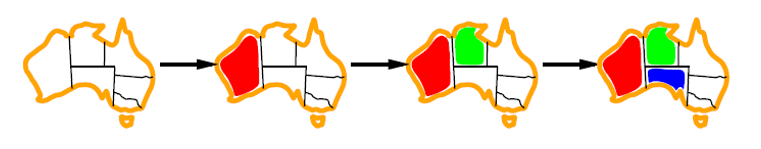
\includegraphics[width=12cm, keepaspectratio]{img/impr_fewest_legal_values.png}
        \label{fig:fewest_legal_values}
    \end{figure}
    \item si sceglie la variabile con \textbf{più vincoli possibili} (degree heuristic) sulle variabili rimanenti.
    \begin{figure}[H]
    	\centering
        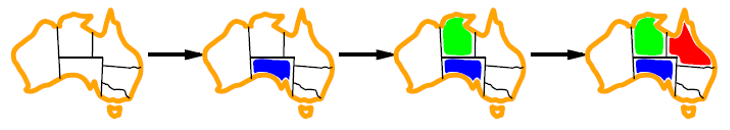
\includegraphics[width=12cm, keepaspectratio]{img/most_constraints.png}
        \label{fig:most_costraint}
    \end{figure}
    \item data una variabile, si sceglie \textbf{il valore meno vincolante} (least-constraining-value), quello che esclude il minor numero di valori nelle restanti variabili.
    \begin{figure}[H]
    	\centering
        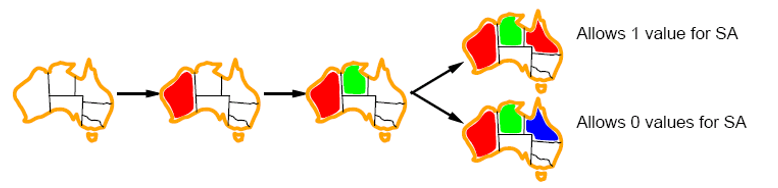
\includegraphics[width=13cm, keepaspectratio]{img/least_constraining_value.png}
        \label{fig:least_constraining_value}
    \end{figure}
\end{itemize}

\section{Propagazione delle informazioni attraverso vincoli}
Finora il nostro algoritmo di ricerca considera i vincoli su una variabile solo nel momento in cui il variabile viene scelta da SELECT-UNASSIGNED-VARIABLE. Ma guardando alcuni dei
vincoli all'inizio della ricerca, o anche prima dell'inizio della ricerca, possiamo drasticamente ridurre lo spazio di ricerca.

\subsection{Forward Checking}

Un modo per fare un uso migliore dei vincoli durante la ricerca è chiamato \textbf{forward checking}(controllo in avanti). Ogni volta che viene assegnata una variabile X, il processo di forward checking esamina ogni variabile non assegnata Y che è connessa a X da un vincolo e cancella dal dominio di Y qualsiasi valore non coerente con il valore scelto per X.
\begin{figure}[H]
    \centering
    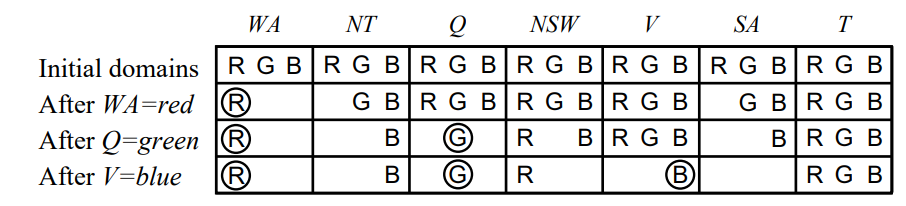
\includegraphics[width=13cm, keepaspectratio]{img/forward_checking.png}
    \caption{Forward checking applicata a Map-colouring problem.}\label{fig:forward_checking}
\end{figure}

Ci sono due punti importanti da notare su questo esempio. Innanzitutto, si noti che dopo aver assegnato WA = rosso e Q = verde, i domini di NT e SA
sono ridotti ad un unico valore; abbiamo eliminato del tutto la ramificazione su queste variabili di propagare le informazioni da WA e Q. L'euristica MRV, che è un partner ovvio per il controllo in avanti, selezionerebbe automaticamente SA e NT successivamente.

\subsection{Constraint propagation}
Sebbene il forward checking rilevi molte incoerenze, non le rileva tutte. Per esempio, consideriamo la terza riga della Figura \ref{fig:forward_checking}. Essa mostra che quando WA è rosso e Q è verde, sia NT che SA sono costretti a essere blu ma questo non è possibile perchè sono due zone vicine. Il forward checking non rileva questo come un'incoerenza, perché non guarda abbastanza avanti. La propagazione del vincolo (constraint propagation) è il termine generale per propagare le implicazioni di un vincolo su una variabile su altre variabili; in questo caso dobbiamo propagare da WA e Q su NT e SA, e quindi sul vincolo tra NT e SA per rilevare l'incoerenza. 

\subsubsection{Domain Consistency} L'idea di \textbf{arc consistency} fornisce un metodo veloce di propagazione dei vincoli sostanzialmente più forte del forward checking.
Una variabile è \textbf{consistente al dominio} (domain consistent) se nessun valore del dominio del nodo è è dichiarato impossibile da uno qualsiasi dei vincoli. L'idea è di "potare" il più possibile prima di selezionare un valore per le variabili. La domain consistency è stata definita solo per i vincoli che coinvolgono una sola variabile. Quando i vincoli sono binari, possiamo usare gli archi per indicare che un vincolo vale tra una coppia di variabili:
\begin{itemize}
    \item un \textbf{nodo} per ogni variabile;
    \item un \textbf{arco} per ogni vincolo.
\end{itemize}

\paragraph{Node Consistency.} In questo caso tutti i vincoli sono unari, le variabili sono rappresentate da dei \textbf{vertici}. Il vertice è \textbf{node consistent} se ogni valore nel dominio delle variabili soddisfa tutti i vincoli unari imposti sulla variabile X. Spesso vengono rappresentati come un cappio o arco che ritorna sullo stesso nodo. 
\begin{figure}[H]
    \centering
    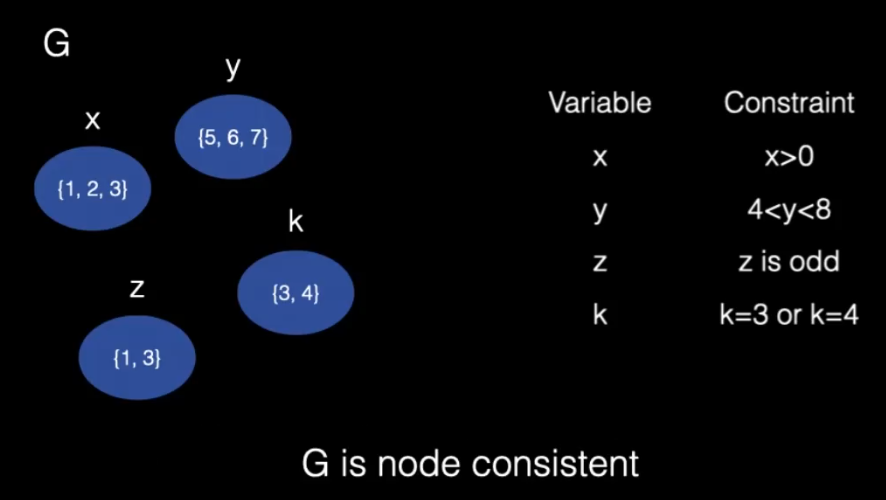
\includegraphics[width=13cm, keepaspectratio]{img/node_consistency.png}
    \caption{Esempio grafo node consistent.}\label{fig:node_consistency}
\end{figure}

\paragraph{Arc Consistency.} 
Quando tutti i vincoli sono binari si parla di \textbf{arc consistency}. Un arco (u,c) è consistente se per ogni valore x del dominio dom(u) esiste un valore y nel dom(v) tale che un assegnamento u=x e v=y soddisfa tutti i vincoli binari che coinvolgono sia u che v.

\subparagraph{Arc Consistency Algorihtm.} Per fare diventare un arco (u,v) consistente si cancellano tutti i valori x dal dom(u) che sono incosistenti con tutti i valori in dom(v). Restituisce true se è stata fatta una modifica al dominio di u.
\begin{figure}[H]
    \centering
    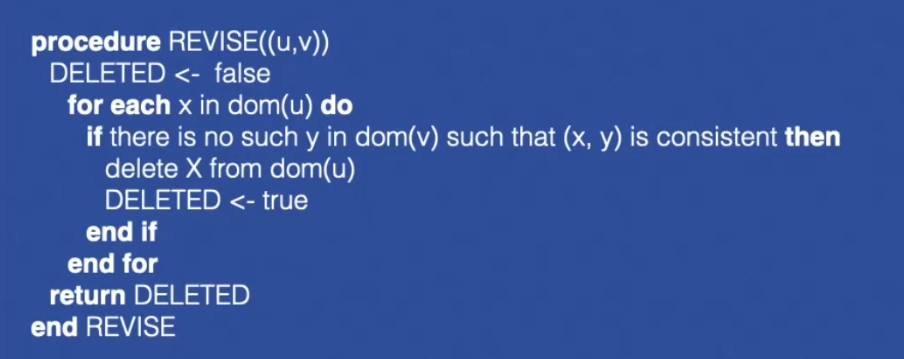
\includegraphics[width=13cm, keepaspectratio]{img/arc_consistency.png}
    \caption{Procedura REVISE.}\label{fig:arc_consistency}
\end{figure}


\subparagraph{AC-1} Un singolo passo dell'agoritmo REVISE non è sufficiente. L'algoritmo base per arc consistecy è AC-1, il quale esegue l'algoritmo REVISE finchè il dominio delle variabili cambia. In questo si ripete la procedura REVISE ogni volta che viene modificato un valore in un dominio.
\begin{figure}[H]
    \centering
    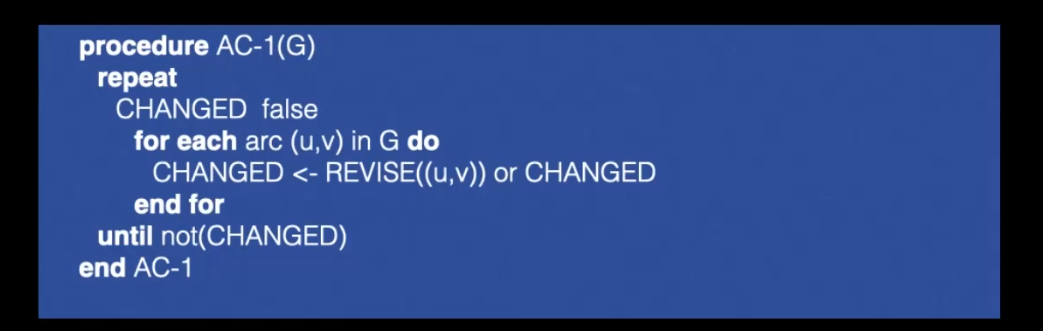
\includegraphics[width=13cm, keepaspectratio]{img/ac1_real.png}
    \caption{Algoritmo AC-1.}\label{fig:ac1}
\end{figure}
Una sola revisione riuscita di un arco su una particolare iterazione causa la revisione di tutti gli archi nella prossima iterazione anche se gli archi non sono influenzati dal cambiamento.

\subparagraph{AC-2}
AC-2 è un algoritmo che può fare arc consistecy in un solo passo attraverso i nodi. Il risultato è ottenuto passando per i nodi in un ordine numerico:
\begin{itemize}
    \item allegare ad un nodo tutti i valori che non sono in conflitto con i nodi precedentemente assegnati;
    \item Guardando i vicini di questo nodo che sono stati già valutati; se un valore non ha un'assegnazione corrispondente per lo stesso arco, eliminalo;
    \item Ogni volta che qualsiasi valore è cancellato da un arco, guarda ai suoi vicini a sua volta, e si controlla se un loro valore può essere eliminato. Se può essere eliminato, si continua il processo iterativamente finchè non ci sono più cambiamenti che possono essere fatti. Poi si prosegue con gli altri archi.
\end{itemize}
In sostanza si sceglie un ordine fra i nodi, prendiamo ad esempio y come primo e controlliamo tutti i vincoli fra y e k se c'è qualche valore di dom(y) che va in conflitto allora si elimina. Stessa cosa si per l'arco (x,y) se si fa qualche modifica si rimette in coda l'arco in modo da controllare se ci sono altre modifiche da fare. Se un valore b del nodo i è rimosso allora si aggiunge tutti (k,i) alla coda Q, per il controllo degli archi.
\begin{figure}[H]
    \centering
    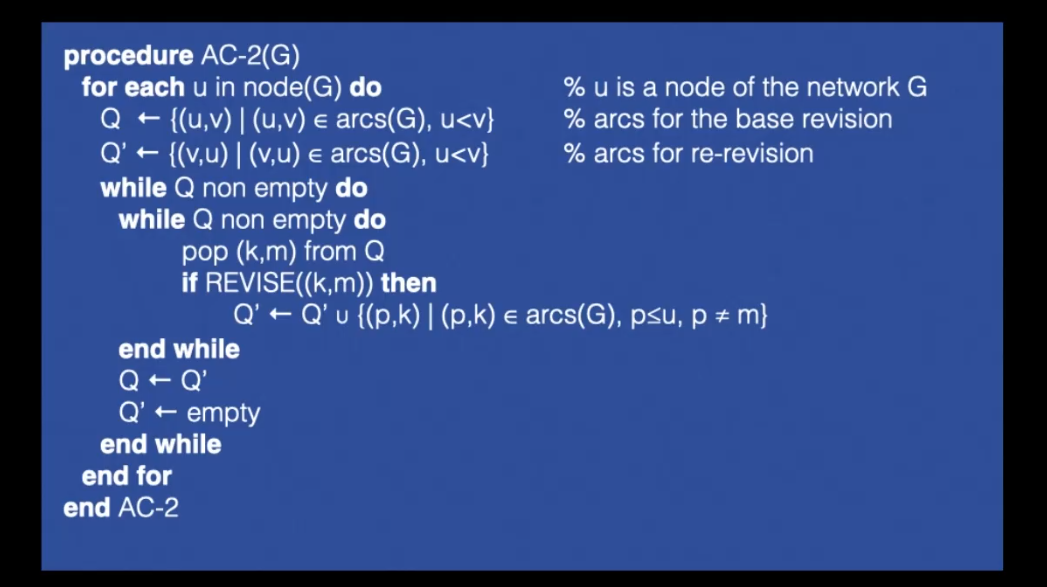
\includegraphics[width=13cm, keepaspectratio]{img/ac-2.png}
    \caption{Algoritmo AC-2.}\label{fig:ac2}
\end{figure}

\subparagraph{AC-3}
AC-3 è un miglioramento di AC-2, alcuni di essi possono essere già essere nella coda Q. Se è così allora non dovrebbero essere inseriti di nuovo. 
\begin{figure}[H]
    \centering
    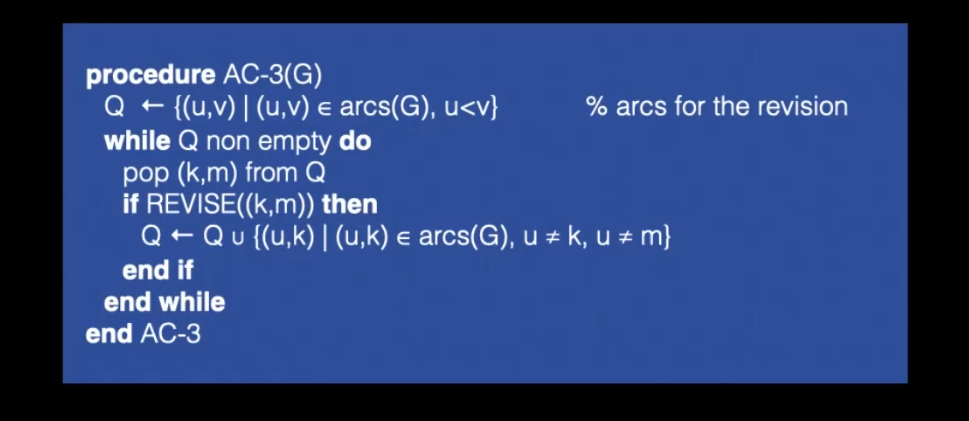
\includegraphics[width=13cm, keepaspectratio]{img/ac3.png}
    \caption{Algoritmo AC-3.}\label{fig:ac3}
\end{figure}
In sostanza si prende un arco dalla coda Q, si fa la REVISE, se faccio una modifica allora si aggiunge alla coda Q tutti gli archi (u,k) che non sono stati già controllati ovvero $u \neq k$ e $u\neq m$.
\section{Soft Constraint Satisfaction Problems}
I vincoli che abbiamo visto in precedenza sono dei vincoli \textbf{assoluti}, la cui violazione esclude una possibile soluzione. Molti dei problemi CSP reali includono i vincoli \textbf{preference} i quali indicano quali soluzioni sono preferite. Per esempio in un problema di timetable in università ci potrebbe essere il professore X che preferisce insegnare la mattina mentre il professore Y preferisce insegnare il pomeriggio. Un timetable dove il prof X insegna alle 14 e il prof Y alle 9 potrebbe essere una soluzione, ma non è quella ottimale viste le preferenze. I vincoli sulle preferenze possono essere codificati spesso come dei \textbf{costi} applicati sugli assegnamenti individuali delle variabili. Riprendendo l'esempio di prima possiamo dare all'assegnamento prof X = (lezione alle 14) un costo di 2, mentre all'assegnamento prof X = (lezione alle 9) un costo di 1. In questo modo si cerca fra le possibili soluzioni quella ottimale andando a minimizzare (o massimizzare...) il costo della soluzione. \\
Supponiamo di avere un problema di colorazione del grafo e cerchiamo di trovare una soluzione ottimale. 
\begin{figure}[H]
    \centering
    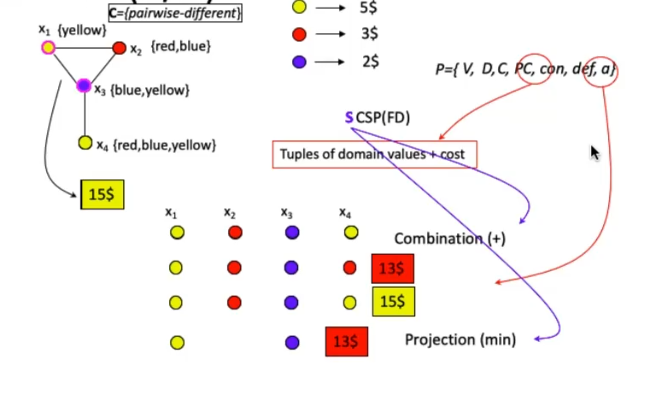
\includegraphics[width=12cm, keepaspectratio]{img/scsp_grafo.png}
    \caption{Esempio di SCSP su grafo.}\label{fig:scps_grafo}
\end{figure}

Partiamo riprendendo la definizione di un CSP, esso è definito come P=\{V,D,C,PC,con,def,a\} i quali indicano:
\begin{itemize}
    \item V= insieme delle variabili;
    \item D= insieme dei domini associati alle variabili;
    \item C= insieme di vincoli, definito come l'associazione variabile-vincolo ovvero quali variabili sono coinvolte in quale vincolo;
    \item PC= sono i vincoli primitivi e variano in base al vincolo e al dominio. A seconda del tipo di vincolo che possiamo avere i primitivi possono essere diversi, esempio se lavoro sugli interi esso conterrà vincoli con gli operatori <,>,= . Sostanzialmente esso indica i tipi di vincoli che posso usare se lavoro su un dominio specifico. Inoltre indicano se il vincolo è implicito (tutti i colori diversi) o esplicito (valgono le coppie <r,g,b>, <g,r,b>, …).
    \item con= funzione che definisce quali variabili sono coinvolte in quale vincolo, essa dato un vincolo restituisce le variabili che sono connesse a questo;
    \item def= funzione che indica quali sono i valori del dominio possibili per una specifica variabile. In un SCSP questa funzione oltre a dire i valori possibili per una variabile deve indicare anche il costo associato a quei valori, nell'esempio in Figura \ref{fig:scps_grafo} se passiamo in input alla funzione def la variabile $x_1$ essa ci ritornerà come valori possibile il colore giallo con costo 5\$. Questa è la differenza con la funzione def di un problema CSP.
    \item a= sottoinsieme di V contenente tutte le variabili interessate nella soluzione del SCSP, ad esempio nel caso del grafo abbiamo che le variabili che ci interessano per la soluzione ottimale sono solo $x_1$ e $x_3$, non tutte quante.
\end{itemize}
Nell'esempio in Figura \ref{fig:scps_grafo} i vincoli binari sono hard, perché la soluzione richiede per forza che i nodi collegati abbiamo colori diversi sennò si violano i vincoli, mentre i vincoli unari (quelli del costo sul colore) sono soft.
Nel caso di un CSP quando utilizziamo un algoritmo di ricerca per trovare una soluzione esso si può fermare alla prima soluzione che trova oppure, se richiesto, le cerca tutte quante. Nel caso di SCSP siamo costretti a trovare tutte le possibili soluzioni in modo da scegliere la migliore.
Normalmente si utilizzano due operazioni per trovare la soluzione ottimale in un SCSP:
\begin{itemize}
    \item \textbf{Combinazione (+)}: dove metto insieme tutti gli assegnamenti, combinando i vincoli, quindi si calcola anche il costo totale ad esempio con l'operazione di somma;
    \item \textbf{Proiezione ($\times$)}: operazione di scelta della soluzione migliore data dalla combinazione in base al minimo o al massimo del costo.
\end{itemize}
\subsection{Semiring}
Un semiring <A,+,$\times$,0,1> è una struttura costituita dai seguenti simboli:
\begin{itemize}
    \item \textbf{A}: l'insieme degli elementi che mi rappresentano i costi, quindi il dominio dei costi, esso può essere l'insieme dei reali oppure un intervallo specifico [0,1]
    \item \textbf{+}: operatore di proiezione, usato per fare la scelta fra le soluzioni trovate dalla combinazione, può essere il minimo o massimo. Possiamo definire alcune proprietà:
    \begin{itemize}
        \item \textbf{idempotente}: se faccio a+a dove +=minimo il risultato è sempre a, quando un operatore è idempotente è possibile definire un ordinamento ovvero 
        \[ a \leq b \text{ b è meglio di a } \iff a+b=b\]
    \end{itemize}
    \item \textbf{$\times$}: operatore di combinazione, utilizzato per combinare i vincoli, può essere somma,moltiplicazione etc... dipende dal problema. Possiamo definire alcune proprietà:
    \begin{itemize}
        \item \textbf{commutativa}: si considera il set di vincoli invece delle tuple.
    \end{itemize}
    \item \textbf{0}: rappresenta il valore minimo (peggiore) dell'insieme A, ovvero il bottom sotto il quale non si può andare, per l'intervallo [0,1] è 0;
    \item \textbf{1}: rappresenta il valore massimo (migliore) di A, il top, per l'intervallo [0,1] è 1. 
\end{itemize}
Tutti questi che abbiamo visto sono simboli quindi quando si utilizza l'operatore + non si ci si riferisce alla somma ma a un operatore per la proiezione che potrebbe essere minimo o massimo o or.

\subsubsection{Differenti tipi di semiring}
Esistono diversi tipi di semiring:
\begin{itemize}
    \item \textbf{Probabilistico}: <$\Re^+$, min, +, $+\infty$, 0> si minimizza la probabilità;
    \item \textbf{Weighted}: <[0,1],max,x,0,1> massimo il costo dato dalla combinazione, dove si fa il prodotto;
    \item \textbf{Fuzzy}: <[0,1],max,min,0,1>;
    \item \textbf{Classical}: <\{false,true\}, $\vee$, $ \wedge$, false, true>
\end{itemize}

\subsection{Local consistency}
Cerchiamo ora di vedere se è possibile applicare una tecnica di constraint propagation come arc consistency ai problemi SCSP in modo da rendere più efficiente la ricerca della soluzione. 
\subparagraph{Teorema dell'estensività} Se tolgo dei vincoli da un problema SCSP, la soluzione migliore perchè si moltiplica di meno (meno calcoli da fare),se li aggiungo la soluzione peggiora. Togliere vincoli vuol dire \textbf{rilassare} il problema.
\\
Se l'operatore x è idempotente allora possiamo applicare arc consistency, un esempio di operatore idempotente è il minimo se facciamo
\[1\times1= 2 \text{ dove $\times$ = somma}\]
\[1\times1= 1 \text{ se $\times$ = minimo}\]
Nei Semiring Fuzzy è possibile applicare arc consistency perchè $\times$ = min. Vediamo un esempio. 
\begin{figure}[H]
    \centering
    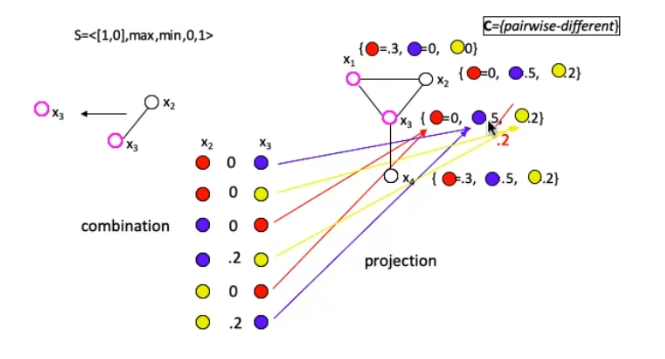
\includegraphics[width=12cm, keepaspectratio]{img/SCSP_arc_consistency.png}
    \caption{SCSP arc-consistency.}\label{fig:SCSP_arc_consistency}
\end{figure}
Nel caso dei SCSP quando si fa arc-consistency non si va a togliere elementi dal dominio ma si vanno a modificare i costi associati a quell'assegnamento. Ad esempio per il vincolo ($x_3$, $x_2$) andiamo a combinare tutti i vincoli e riportiamo tutte le coppie con i relativi costi, in questo caso si prende il minimo fra i due valori. E poi si proietta su $x_3$ i valori che abbiamo trovato e andiamo a modificare i costi associati ai colori, per $x_3$ = rosso e $x_3$ = giallo non cambiano perchè il $max_{rosso}(0,0) = 0$ e $max_{giallo}(0,0.2) = 0.2$ mentre per il blu abbiamo $max_{blue}(0,0.2) = 0.2$ quindi $x_3= 0.5 \xrightarrow{}0.2$.
\\
DA COMPLETARE 
\\
\chapter{Argumentation Framework}
\paragraph{Argumentation Framework.}Un argumentation framework (AF) è una coppia (A,R) dove 
\begin{itemize}
    \item A è un set di argomentazioni 
    \item $R \subseteq  A\times  A$ è una relazione rappresentante gli "attacchi" ("sconfitte")
\end{itemize}

\begin{center}
    F(\{a,b,c,d,e\}, \{(a,b),(c,b),(c,d),(d,c),(d,e),(e,e)\})
\end{center}
\begin{figure}[H]
    \centering
    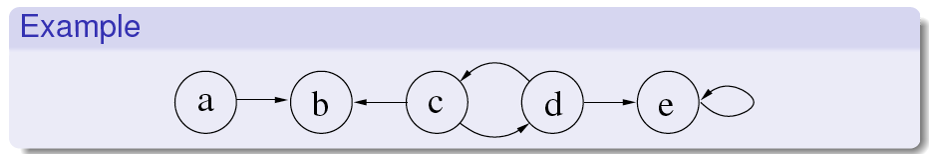
\includegraphics[width=12cm, keepaspectratio]{img/arg_fram.png}
    \caption{Argumentation framework.}\label{fig:arg_fram}
\end{figure}
Si ha un attacco quando si ha un'espressione logica (frase, dato...) che è in contraddizione con un'altra. Gli attacchi possono essere anche pesati, essi possono dipendere anche da chi ha detto quella frase.
\begin{figure}[H]
    \centering
    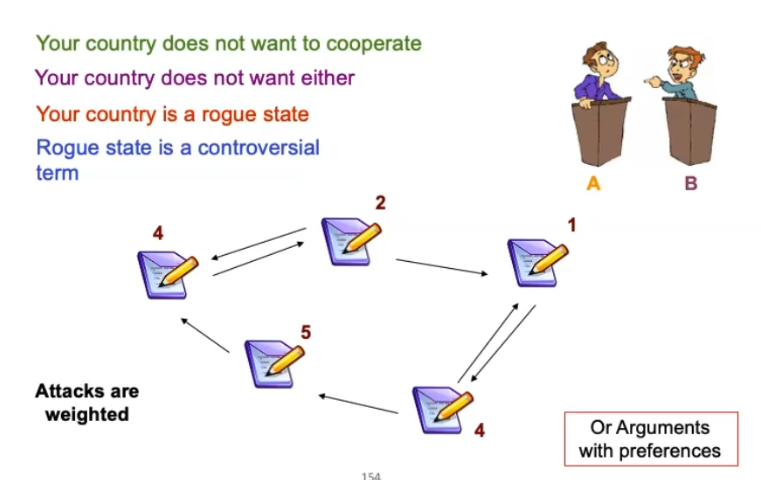
\includegraphics[width=12cm, keepaspectratio]{img/es_arg_fram.png}
    \caption{Esempio di argumentation framework.}\label{fig:es_arg_fram}
\end{figure}
Ci possono essere anche casi in cui è noto chi dice l'argomento e altri in cui non lo è. Per quest'ultima vogliamo selezionare gli argomenti che sono più validi rispetto agli altri, ad esempio in Figura \ref{fig:es_arg_fram} il 4 e il 2 sembrano buoni argomenti perchè attaccano gli altri e contrattaccano nel caso siano attaccati. Lo scopo è di definire dei criteri per trovare gli argomenti più forti, validi (che stanno "in piedi da soli"), in modo da selezione i conflitti che riescono a sopportare gli attacchi dall'esterno. 
\begin{figure}[H]
    \centering
    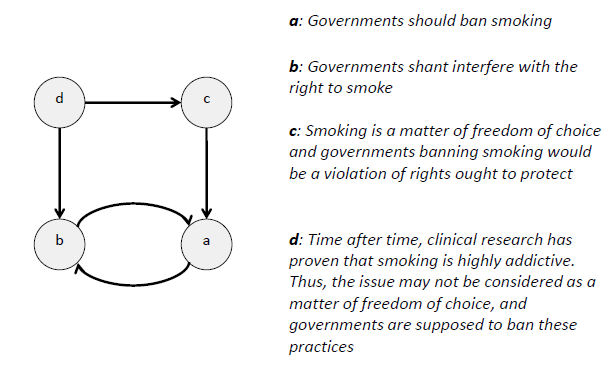
\includegraphics[width=13cm, keepaspectratio]{img/es_2_arg_fram.png}
    \caption{Altro esempio di argumentation framework.}\label{fig:es_2_arg_fram}
\end{figure}
Dobbiamo trovare gli argomenti che "stanno bene insieme", la prima nozione di questo tipo è un insieme di argomenti senza conflitti. 

\subsection{Extension-Based Semantics}
Queste solo le semantiche (criteri) che vanno a studiare i sottoinsiemi di argomenti per stabilire l'accettabilità degli stessi, ovvero se un argomento è un'estensione accettabile altrimenti viene rigettato.

\paragraph{Conflit-free extensions.} Dato un AF. F=(A,R). Un insieme $S\subseteq A$ è \textbf{conflict-free} in F, se, per ogni $a,b \in S ,(a,b) \notin R$.
\begin{figure}[H]
    \centering
    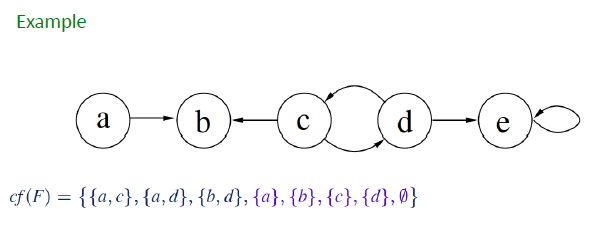
\includegraphics[width=13cm, keepaspectratio]{img/es_conflict_free.png}
    \caption{Esempio insieme conflict-free.}\label{fig:es_conflict_free}
\end{figure}
In questo caso andiamo a scegliere come coppie gli argomenti che non sono in conflitto (quindi che non si attaccano) fra di loro, (\{a,c\},\{a,d\} ma non \{a,b\}), e anche i singoli argomenti tranne e poichè esso si contraddice da solo visto che ha un cappio. 

\paragraph{Insiemi Ammissibili (Admissible).} Dato AF, F=(A,R). Un insieme $S \subseteq A$ è \textbf{ammissibile} in F, se 
\begin{itemize}
    \item S è conflict-free in F
    \item ogni $a\in S$ è difesa da S in F
    \begin{itemize}
        \item  $a\in A$ è difesa da S in F, se per ogni $b\in A$ con $(b,a) \in R$, esiste una $c\in S$, tale che $(c,b)\in R $
    \end{itemize}
\end{itemize}
Quindi gli insiemi admissible sono quelli senza conflitti e gli argomenti si difendono.
\begin{figure}[H]
    \centering
    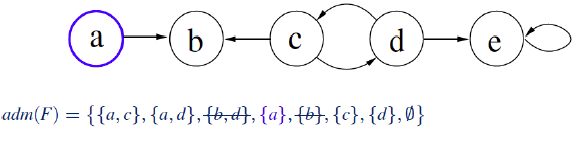
\includegraphics[width=13cm, keepaspectratio]{img/es_insieme_ammissibile.png}
    \caption{Esempio insieme ammissibile.}\label{fig:es_insieme_ammissibile}
\end{figure}
Non è necessario che sia lo stesso argomento a difendersi da altri attacchi, ad esempio in questo caso ,supponendo che non ci sia a, b è attaccato da c ma  se prendo d lui oltre che difendere se stesso da c (poichè attaccato) difende anche b. Guardando la definizione di difesa, un argomento a è difeso da un argomento b, $(b,a) \in R$, nel momento in cui esiste un argomento c tale che c attacca b, $(c,b) \in R$. Il sottoinsieme \{b,d\} non viene scelto poichè d è attaccato da c ma a si difende a sua volta contrattaccando, mentre b è attaccato sia da a che c, nel primo caso nessuno lo difende nel secondo d difende b perchè attacca c.

\paragraph{Insieme Completo (tutti difesi).} Dato un AF, F=(A,R). Un insieme $S \subseteq A$ è \textbf{completo} in F, se 
\begin{itemize}
    \item S è ammissibile in F
    \item ogni $a\in A$ difeso da S in F è contenuto in S
    \begin{itemize}
        \item $a\in A$ è difeso da S in F, se per ogni $b\in A$ con $(b,a) \in R$, esiste una $c\in S$, tale che $(c,b)\in R$.
    \end{itemize}
\end{itemize}
\begin{figure}[H]
    \centering
    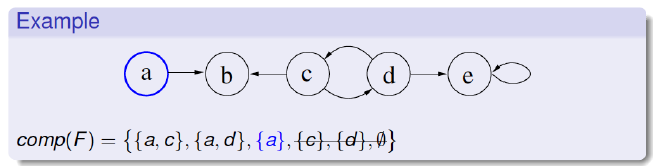
\includegraphics[width=13cm, keepaspectratio]{img/es_set_complete.png}
    \caption{Esempio insieme completo.}\label{fig:es_insieme_completo}
\end{figure}
Quindi un insieme complete contiene tutti gli insiemi ammissibili e anche tutti gli argomenti che sono difesi.

\paragraph{Grounded (scettica).} Dato un AF F=(A,R). Un insieme $S \subseteq A$ è \textbf{grounded} in F, se 
\begin{itemize}
    \item S è completo in F
    \item per ogni $T \subseteq A$ completo in $F,T \nsubseteq  S$.
\end{itemize}

\begin{figure}[H]
    \centering
    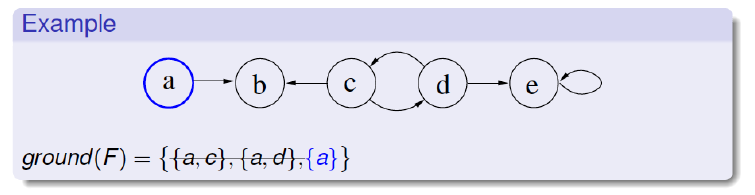
\includegraphics[width=13cm, keepaspectratio]{img/es_grounded.png}
    \caption{Esempio grounded.}\label{fig:es_insieme_grounded}
\end{figure}
Sceglie tra gli argomenti che sono nella complete, gli argomenti che compaiono in tutte le estensioni, è una semantica scettica perchè vuole essere sicuro che gli argomenti che sceglie provengano da una decisione prudente. 

\paragraph{Preferred.} Dato un AF, F= (A,R). Un insieme $S\subseteq A$ è \textbf{preferito} in F, se 
\begin{itemize}
    \item S è ammissibile in F
    \item per ogni $T\subseteq A$ ammissibile in T, $S\nsubseteq T$
\end{itemize}


\begin{figure}[H]
    \centering
    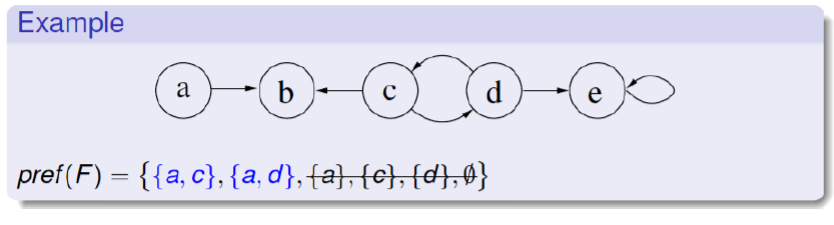
\includegraphics[width=13cm, keepaspectratio]{img/es_preferred.png}
    \caption{Esempio preferred.}\label{fig:es_insieme_preferred}
\end{figure}

Al contrario di grounded dove si andava a scegliere l'insieme con l'elemento in comune con gli altri insieme, in questo caso si va a scegliere tra gli insiemi ammissibili quelli che sono più grandi. Da notare che si sceglie tra gli insiemi ammissibili ma si può dimostrare che si può scegliere da quelli complete.

\paragraph{Stable.} Dato un AF, F= (A,R). Un insieme $S\subseteq A$ è \textbf{stabile} in F, se
\begin{itemize}
    \item S è conflict-free in F
    \item per ogni $a\in A\setminus S$, esiste una $b\in S$, tale che $(b,a)\in R$. 
\end{itemize}

\begin{figure}[H]
    \centering
    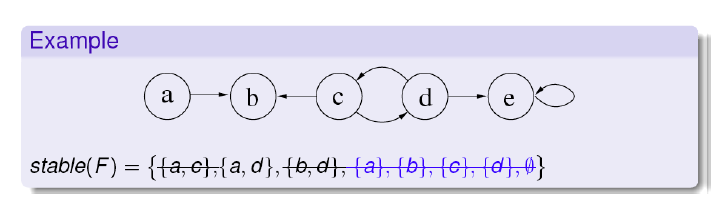
\includegraphics[width=13cm, keepaspectratio]{img/es_stable.png}
    \caption{Esempio insieme stable.}\label{fig:es_insieme_stable}
\end{figure}
In questo caso si sceglie l'insieme i quali elementi attaccano tutti gli elementi fuori dall'insieme conflict-free, ad esempio \{a,c\} non si prende perchè a attacca b e c attacca d e b ma nessuno dei due attacca e. Mentre nell'insieme \{a,d\} a attacca b e d attacca sia c che e. Esiste anche una semantica \textbf{semi-stabile} la quale nel caso cui esista un insieme stabile allora essa coincide con quest'ultimo ma quando non c'è la stabile allora sceglie tra gli insieme preffered quelli che ne attaccano di più tra gli insiemi fuori a quest'ultimo. L'obiettivo della semantica stabile è di avere  cardinalità più grande possibile e di attaccare tutti gli insiemi fuori.

\subsubsection{Complessità}
La complessità è descritta da due valori:
\begin{itemize}
    \item \textbf{Cred}: (credulous) rappresenta il costo associato all'operazione di controllo sulle semantiche, si controlla se un determinato insieme contiene un argomento passato;
    \item \textbf{Skept}: (scettico) controlla se un argomento è incluso in tutte le estensioni.
\end{itemize}
Manca seconda parte
\subsection{Labelling-Based Semantics}
\subsubsection{Reinstatement Labelling}
Finora abbiamo visto delle estensioni in cui gli argomenti venivano accettati (validi, quelli che si trovavano all'interno delle estensioni) o rigettati. Con le labelling semantics manteniamo queste due sfumature e ne aggiungo un'altra ovvero gli argomenti vengono suddivisi in:
\begin{itemize}
    \item \textbf{IN}: argomenti accettati, sono IN se sono attaccati solo da argomenti OUT;
    \item \textbf{OUT}: argomenti rigettati, sono OUT se sono attaccati solo da argomenti IN;
    \item \textbf{UNDEC}: altrimenti, tutto il resto .
\end{itemize}
\begin{figure}[H]
    \centering
    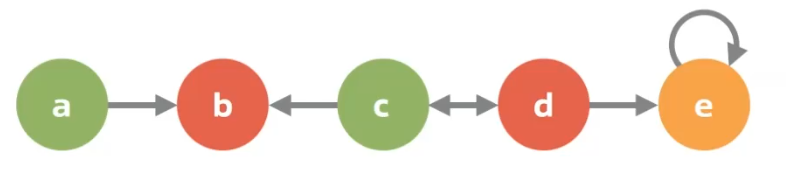
\includegraphics[width=13cm, keepaspectratio]{img/labelling_semantics_es.png}
    \caption{Esempio Reinstatement Labelling .}\label{fig:es_Reinstatement_Labelling}
\end{figure}

\paragraph{Conflict-free.}
Per ogni $a \in A$ si ha che:
\begin{itemize}
    \item se a è etichettata IN allora non ha un attaccante che è IN e
    \item se a è etichettata OUT allora ha almeno un attaccante che è IN
\end{itemize}
La Figura \ref{fig:es_Reinstatement_Labelling} è conflict-free perchè valgono le due regole citate per tutti gli argomenti. 

\begin{figure}[H]
    \centering
    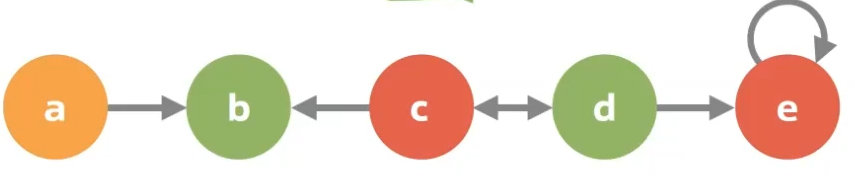
\includegraphics[width=13cm, keepaspectratio]{img/es_conflict_free_labelling.png}
    \caption{Esempio conflict-free con labelling .}\label{fig:es_conflict_free}
\end{figure}
Anche in questo caso abbiamo un insieme conflict-free.
\begin{figure}[H]
    \centering
    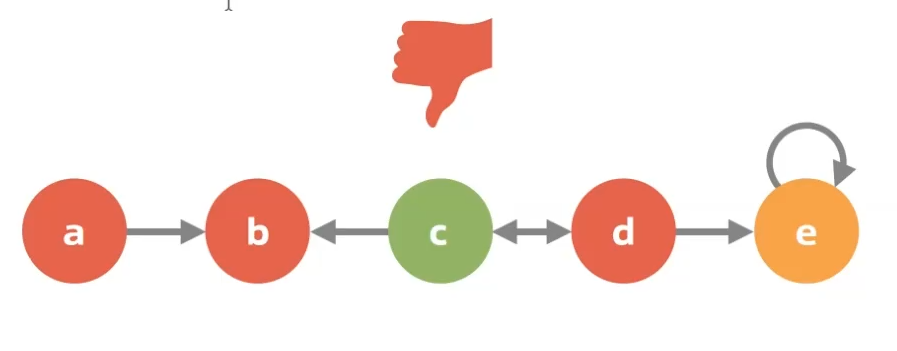
\includegraphics[width=13cm, keepaspectratio]{img/es_no_conflict_free_labelling.png}
    \caption{Esempio no conflict-free con labelling .}\label{fig:es_noconflict_free}
\end{figure}
In questo ultimo esempio non abbiamo un insieme conflict-free perchè a viene considerato OUT, quindi rigettato, anche se non viene attaccato da nessuno e infatti non ci sono attaccanti IN per quest'ultimo.

\paragraph{Admissible.}
Per ogni $a \in A$ si ha che:
\begin{itemize}
    \item se a è etichettata IN allora tutti gli attaccanti sono OUT e
    \item se a è etichettata OUT allora ha almeno un attaccante che è IN
\end{itemize}
L'interpretazione che possiamo dare alla prima regola è che un argomento IN è accettato come nell'insieme admissible se i suoi attaccati sono tutti sconfitti.
Riprendo l'esempio in Figura \ref{fig:es_Reinstatement_Labelling} è un insieme admissible, poichè a non è attaccato da nessuno quindi la prima condizione è vera e anche per c poichè essa è attaccata solo da argomenti OUT ovvero d. Anche l'esempio in Figura \ref{fig:es_conflict_free} è admissible.

\paragraph{Completo.}
Per ogni $a \in A$ si ha che:
\begin{itemize}
    \item a è etichettata IN \textbf{se e solo} se tutti gli attaccanti sono OUT e
    \item a è etichettata OUT\textbf{ se e solo se} ha almeno un attaccante che è IN
\end{itemize}
Quesro vuol dire che se un argomento è difeso deve stare per forza dentro l'estensione. Perciò un attaccante è IN se ha solo attaccanti OUT e viceversa se un argomento ha solo attaccanti OUT allora è per forza etichettato come IN. Stessa discorso vale per la seconda regola, dobbiamo vederla come divisa in due parti la parte di sinistra e di destra al se e solo. 

\begin{figure}[H]
    \centering
    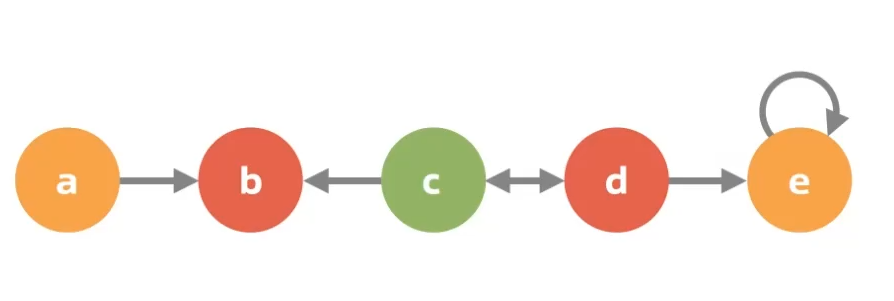
\includegraphics[width=13cm, keepaspectratio]{img/es_no_complete_labelling.png}
    \caption{Esempio no complete con labelling .}\label{fig:es_no_complete_labelling}
\end{figure}
In questo esempio non abbiamo un insieme complete perchè l'argomento a che è etichettato come UNDEC non ha attaccanti e quindi dovrebbe essere etichettato come IN.

\begin{figure}[H]
    \centering
    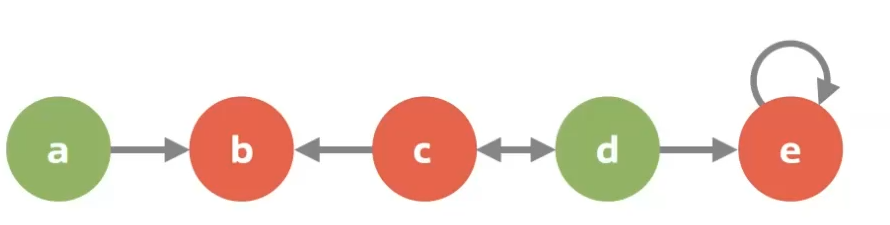
\includegraphics[width=13cm, keepaspectratio]{img/es_complete_labelling.png}
    \caption{Esempio  complete con labelling .}\label{fig:es_no_complete_labelling}
\end{figure}
Ogni etichettatura degli argomenti verifica le regole scritte in precedenza infatti a non ha attaccanti quindi è IN, b ha un attaccante IN quindi è OUT, c ha un attaccante IN quindi è OUT, d ha tutti attaccanti OUT ovvero c e per ultimo e potrebbe essere UNDEC ma essendo che ha almeno un attaccanti IN allora è considerato OUT.

\paragraph{Preferred.}
L'etichettatura
\begin{itemize}
    \item è un insieme complete, e 
    \item l'insieme di argomenti IN è \textbf{massimale} fra tutte le etichette complete.
\end{itemize}
In questo caso si ragiona sulla cardinalità quindi si va a prendere il numero maggiore di argomenti che sono considerati completi. Questa semantica è preferita nel caso in cui si vogliano tirare in ballo più argomenti e sentire più opinioni.

\paragraph{Grounded.}
L'etichettatura
\begin{itemize}
    \item è un insieme complete, e 
    \item l'insieme di argomenti IN è \textbf{minimale} fra tutte le etichette complete.
\end{itemize}
Invece per la grounded si vanno a prendere tutti i labelling complete e si sceglie quello in cui ho meno argomenti IN.

\begin{figure}[H]
    \centering
    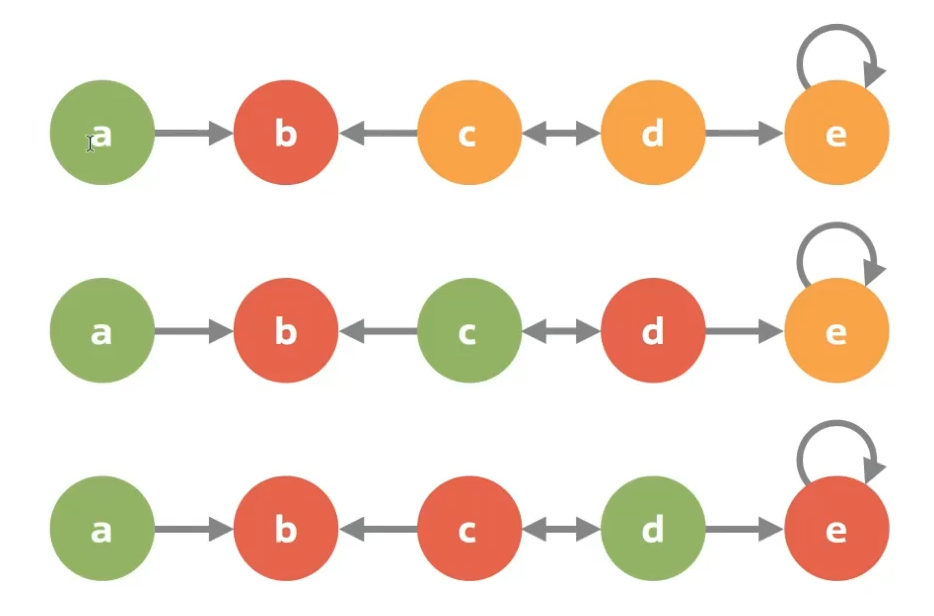
\includegraphics[width=13cm, keepaspectratio]{img/grounded_preferred.png}
    \caption{Esempi insiemi grounded e preferred .}\label{fig:es_grounded_preferred}
\end{figure}
Il primo è un esempio di insieme grounded, gli ultimi due sono preferred. Il secondo insieme è anche grounded perchè le etichette che sono state assegnate come IN sono minimali e massimali, supponiamo di mettere b e d a IN se b è IN non è complete perchè non ha attaccanti OUT stessa cosa vale per d se si etichetta come IN. Se invece assegniamo a c OUT l'insieme non è complete perchè c per essere OUT deve avere almeno un attaccante IN. Lo stesso discorso vale per l'ultimo esempio.
\subsection{Ranking-Based Semantics}
Si trasforma l'AF in un sistema di classificazione, in questo caso con le estensioni non si vanno a scegliere dei sottinsiemi di argomenti ma si a fare una classificazione di quest'ultimi. Per stabilire se un argomento è migliore di un altro si usano dei criteri per studiare la validità, ad esempio possono contare quanti attacchi diretti riceve un argomento o posso misurare la lunghezza dei path da un argomento a un altro etc... 

\paragraph{Categorizer.} Si tratta di una funzione di ranking degli argomenti, la quale assegna un valore agli argomenti controllando quali sono gli attaccanti diretti di questi.

\begin{figure}[H]
    \centering
    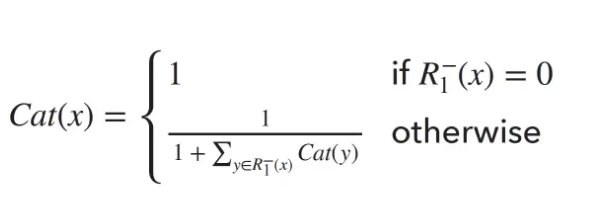
\includegraphics[width=13cm, keepaspectratio]{img/categorizer.png}
    \caption{Funzione categorizer .}\label{fig:fun_categorizer}
\end{figure}
Se un argomento non ha attaccanti $R^{-1}(x) = 0$ allora il valore è 1 sennò è dato dalla formula $\dfrac{1}{1+ \sum_{y \in R^{-1}(x)}^{}Cat(y)}$, questo significa che se ho attaccanti forti allora l'argomento x è debole.
\begin{figure}[H]
    \centering
    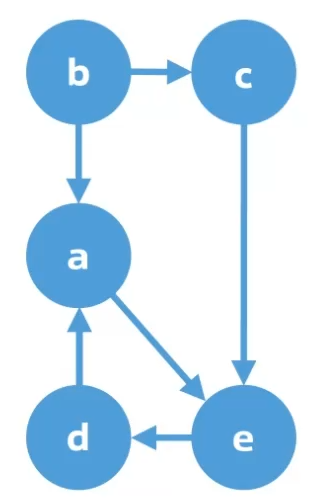
\includegraphics[width=5cm, keepaspectratio]{img/es_categorizer.png}
    \caption{Esempio categorizer .}\label{fig:es_categorizer}
\end{figure}
In questo caso Cat(b)=1 perchè non ha attaccanti e Cat(c)=0.5 perchè è attaccato da b con punteggio 1. Mentre Cat(a)=0.38, Cat(d) =0.65 e Cat(e) = 0.53 quindi la classificazione di questo insieme è 
\[b\succ^{Cat}d\succ^{Cat}e\succ^{Cat}c\succ^{Cat}a\]

\subsection{Graded semantics}
I principi sono simili a quello precedente:
\begin{itemize}
    \item più è grande il numero degli attaccanti su un argomento b, più è debole il livello di giustificazione di b
    \item più è grande il numero di argomenti che difendono a, più è forte il livello di giustificazione di a.
\end{itemize}

\subsubsection{Graded defense}
In questo caso andiamo a ricercare delle partizioni degli argomenti con $d_n^{m}(X)$, il quale è un insieme di argomenti che non hanno almeno m attaccanti che non sono contro attaccati da almeno n argomenti in X. Questo vuol dire che un argomento $a\in d_n^{m}(X)$ se non ci sono almeno m attaccanti che sono difesi da almeno n argomenti.
\begin{figure}[H]
    \centering
    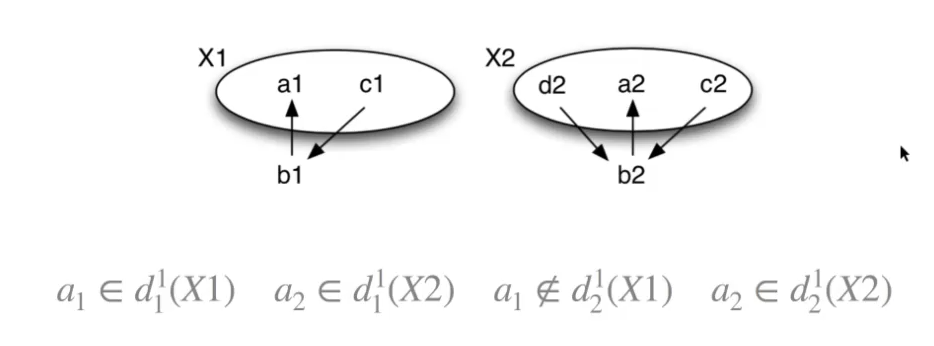
\includegraphics[width=13cm, keepaspectratio]{img/es_graded_defense.png}
    \caption{Esempio graded defense .}\label{fig:es_graded_defense}
\end{figure}

\paragraph{Ranking functions.} Le regole sono:
\begin{itemize}
    \item meno attaccanti ho meglio è
    \item più difensori ho meglio è
\end{itemize}
Scritto in formula 
\[d_n^m \triangleright  d_t^s \iff m \leq s \quad \text{AND} \quad t \leq n\]
Ci possono essere delle funzioni che sono incomparabili. Nell'esempio successivo vediamo che $a_3 \in d_3^3$ e $a_4 \in d_4^4$ quindi dalla regola vista in precedenza ci viene che il n deve essere maggiore quindi fra $a_3$ e $a_4$ è meglio $a_3$ ma allo stesso tempo m deve essere minore quindi $a_4$ è un'argomentazione migliore. Questo porta a una contraddizione perchè non riusciamo a classificare i due argomenti. 
\begin{figure}[H]
    \centering
    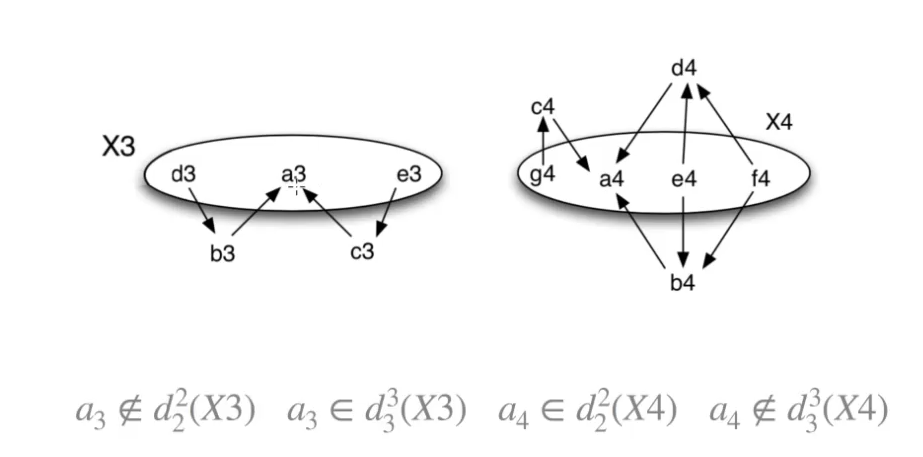
\includegraphics[width=13cm, keepaspectratio]{img/graded_sem_partial_order.png}
    \caption{Esempio graded defense partial order.}\label{fig:es_graded_defense_partial order}
\end{figure}

\begin{figure}[H]
    \centering
    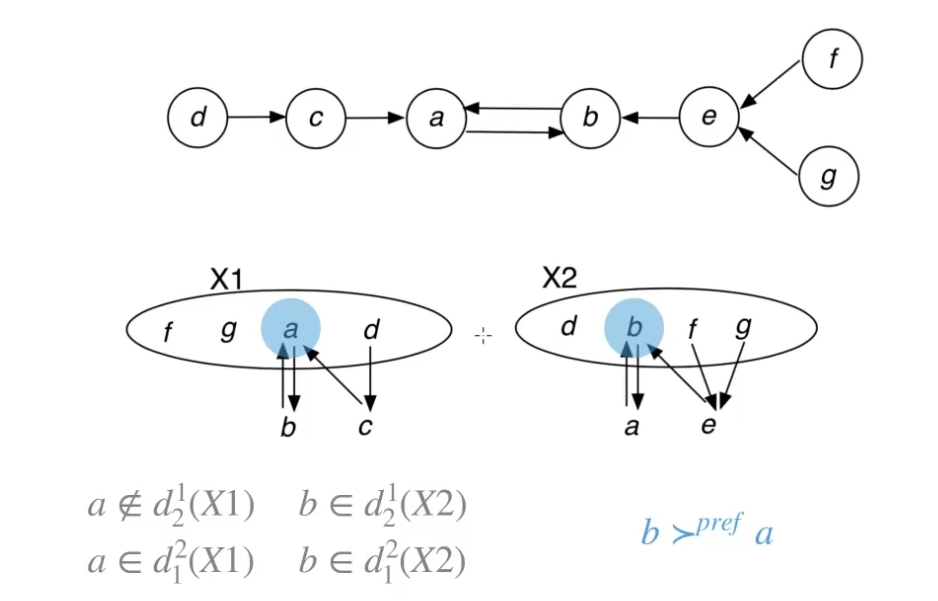
\includegraphics[width=13cm, keepaspectratio]{img/es_fin_graded_semantics.png}
    \caption{Applicazione di graded semantics a AF .}\label{fig:es_fin_graded_semantics}
\end{figure}

 	\newpage
    \chapter{Fondamenti di Calcolo delle Probabilità e Statistica}
In questo Capitolo verranno riportate alcune nozioni base di Probabilità e Statistica applicabili nel campo della simulazione informatica, indispensabili per la costruzione e l’uso di
modelli di simulazione stocastica.

\section{Variabili stocastiche}
Un modello di simulazione è un modello intrinsecamente stocastico. Infatti i valori usati per le variabili di ingresso, di stato iniziale e i parametri sono decisi a partire dal sistema reale attraverso delle misurazioni fisiche, ogni valore appartiene a una distribuzione di probabilità. Perciò abbiamo bisogno di ripassare alcune nozioni base della probabilità in modo da comprendere i valori estratti da queste distribuzioni.\\

Una variabile stocastica o aleatoria $x_i$ rappresenta l'uscita di un'attività casuale. Essa può assumere n differenti valori dato $i ={1,2,...,n}$, ciascuno con una determinata probabilità $p_i(x) = p_1,p_2,...,p_n$.\label{fun_prob} L'insieme di tutte le probabilità è detto \textbf{funzione discreta di probabilità}. Da ricordare che la somma di tutte le singole probabilità da come risultato 1, ovvero:
\[ \sum_{i=1}^{n} p_i(x) = 1\]

\noindent Esse possono essere definite anche nel seguente modo.\\
Uno spazio di probabilità è una tripla $(\Omega, \mathcal{F}, P)$ dove:
\begin{itemize}
    \item $\Omega$ è lo spazio campione, il quale è un insieme di elementi (spesso l'insieme dei possibili esiti);
    \item $\mathcal{F}$ è lo spazio degli eventi, il quale è una famiglia di sottoinsiemi di $\Omega$ che ha le seguenti proprietà:
    \begin{enumerate}
        \item  $\Omega \in \mathcal{F} $,
        \item $A \in \mathcal{F} \Rightarrow \Omega \setminus A \in \mathcal{F}$,
        \item $A,B \in \mathcal{F} \Rightarrow A \cup B \in \mathcal{F} $.
    \end{enumerate}
    \item $P: \mathcal{F} \rightarrow [0,1]$ è la funzione di probabilità (definita come $p(x)$ in \ref{fun_prob}), la quale è una funzione reale con la seguenti proprietà:
    \begin{enumerate}
        \item $P(A) \geq  0 ,\forall \in \mathcal{F}$,
        \item $P(\Omega) = 1$,
        \item $(A, B \in \mathcal{F}) \wedge(A \cap B=\emptyset) \Longrightarrow P(A \cup B)=P(A)+P(B)$.
    \end{enumerate}
\end{itemize}

Dato uno spazio di probabilità, una variabile casuale è una funzione $ X : \Omega \rightarrow \Re$ che ha la seguente proprietà, per ogni reale $r$, $\{\omega \in \Omega: X(\omega) \leq r\} \in \mathcal{F}$. La funzione $F_X(x) = P(X \leq x = P( \{\omega \in \Omega: X(\omega) \leq r\})$, definita sull'insieme dei reali, è detta \textbf{funzione di distribuzione}.
Le variabili stocastiche o casuali vengono utilizzate poiché nei sistemi da simulare spesso si presentano degli eventi non facilmente prevedibili a priori, come ad esempio l'arrivo di clienti ad uno sportello o la quantità di pioggia in una determinata stagione. Perciò tali fenomeni vengono rappresentati tramite queste variabili dalle quali estrarne poi la distribuzione di probabilità.

\paragraph{Esempio} Si consideri il numero di pazienti che si presentano ad un
ambulatorio tra le 9 e le 10 di mattina, e poniamo $\Omega = {0, 1, 2, . . .}$, $\mathcal{F}= 2^\Omega$ ,
e $X(\omega) = \omega$ (la funzione identità). La funzione X così definita è una variabile
casuale, infatti, per ogni reale $r$ è
\[ \{\omega \in \Omega: X(\omega) \leq r\} = \{0,...,\left \lfloor r \right \rfloor\} \in \mathcal{F}\]


\subsection{Funzione densità di probabilità}
La \textbf{funzione densità di probabilità $f(x)$} si utilizza per definire la probabilità di una variabile di assumere uno specifico valore tra infiniti valori , la quale è praticamente nulla, a causa del processo osservato che è continuo. Detto ciò essa si può definire come la probabilità che $ x_1 \leq x \leq x_2$, ovvero che il valore di x sia compreso in intervallo $[x_1, x_2]$, data da:
\begin{align*}
     & p(x_1 \leq x \leq x_2) = \int_{x_1}^{x_2}f(x) d(x)= \\
     &  \int_{-\infty }^{+ \infty} f(x) dx = 1
\end{align*}
   
\subsection{Funzione cumulativa di distribuzione}
La \textbf{funzione cumulativa di distribuzione $F(x)$} definisce la probabilità che un certo valore sia minore o uguale a x, la quale si può descrivere come:
\[ F(x) = \int_{- \infty}^{X}f(x) d(x) \]
Da cui risulta che $0 \leq F(x) \leq 1$ e $p( x_1 \leq x \leq x_2) = F(x_2) - F(x_1)$.

\subsection{Media}
Per una variabile discreta \footnote{Una variabile casuale è detta \textbf{discreta} se l'insieme di valori che può assumere è numerabile.} si definisce il \textbf{valore atteso} o \textbf{media $E(x)$ oppure $\mu_x$} come:
\[ E(x) =  \sum_{i=1}^{n} x_i p_i(x)\]
Si definisce media di una funzione $y=g(x)$:
\[ E(g(x)) = \sum_{i=1}^{n} g(x_i) p_i(x)\]
Per una variabile continua si ha che la media è pari a:
\[ E(x) = \int_{-\infty}^{+ \infty} xf(x)dx = \lambda_1 = \lambda\]
e per una funzione continua y:
\[ E(x) = \int_{-\infty}^{+ \infty} g(x)f(x)dx = \int_{-\infty}^{+ \infty} g(x)dF(x)\]

Altro...

\subsection{Varianza}
Si definisce \textbf{varianza} di x e si indica con $\sigma^2(x)$, è la media degli scarti quadratici rispetto alla media $\mu_x$ e rappresenta una misura di dispersione di x. La sua radice quadrata, $\sigma_x$ è detta \textbf{deviazione standard}. La varianza è definita come 
\[ \sigma^2(x) = E(x-\lambda)^2 = \int_{-\infty}^{+\infty}(x-\lambda)^2 f(x)dx  \]
Da cui si ricava facilmente
\[\sigma^2(x) = E(x^2) - E^2(x)\]
Se x è una \textbf{variabile discreta} si ha
\[ \sigma^2(x) = \sum_{i=1}^{n}(x_i -E(x))^2 \cdot p_i(x)\]
La deviazione standard viene definita come
\[ \sigma(x) = \sqrt{\sigma^2(x)}\]
\subsubsection{Teorema di Beniaymé-Chebychev}
Il Teorema di Beniaymé-Chebychev lega la deviazione standard di x alla probabilità di deviazione dei singoli valori di x della media:
\[ p(\left | x- \lambda \right | \geq k\sigma) \leq \frac{1}{k^2}   \]
 Ovvero, qualunque sia la forma di $f(x)$, la probabilità al di fuori di $\pm k \sigma$ è limitata, $\leq \frac{1}{k^2}$.
 
 \subsection{Funzione di probabilità di due variabili aleatorie} \label{subsec:prob_congiunta}
 In modo analogo al precedente si definisce la funzione di distribuzione $F(X,Y)$ di due variabili aleatorie x e y
 \[ F(X,Y) = p(x \leq X, y \leq Y)\]
 che indica la probabilità che $x \leq X$ ,valore prefissato, e $y \leq Y$. La suddetta funzione è detta anche \textbf{funzione di probabilità congiunta} e scritta $F(x,y)$.
 Da essa possiamo ottenere la definizione di \textbf{densità congiunta di probabilità}. Nel caso di variabili discrete data l'esistenza di un insieme numerabile di punti 
 \[ (X_1, Y_1), (X_1,Y_2),...,(X_2,Y_2),...,(X_i,Y_j)\]
 con associati numeri positivi 
 \[\ p_{11},p_{12},...,p_{21},p_{22},...,p_{ij}\]
\noindent i quali soddisfano la relazione $F(X_h, Y_k) = \sum_{i}^{}\sum_{j}^{}p_{ij}$ con $\sum_{i}^{}\sum_{j}^{}p_{ij}=1$ sommata per tutti gli i e j per i quali $X_i \leq X_h$ e $Y_j \leq Y_k$.
Allora si può definire $p = (x=X_i, y=Y_j) = p_{ij}$ per tutti gli i e j per i quali esistono dei valori delle variabili x e y, assumendo $p_{ij} = 0$ altrove. Quindi la \textbf{funzione discreta di probabilità congiunta} è $f(x_i, y_j) = p_{ij}$ con distribuzione cumulativa $F(x_i,y_j)$.\\
Se invece la funzione F(x,y) è continua si definisce la \textbf{densità congiunta}
\[f(x,y) = \dfrac{\lambda}{\lambda x} \dfrac{\lambda}{\lambda y} F(x,y) \] e quindi
\[F(x,y) = \int_{-\infty}^{y}\int_{-\infty}^{x} f(x,y) dxdy\]
\[ p(a \leq x\leq b , c \leq y \leq d) = \int_{c}^{d}\int_{a}^{b} f(x,y) dxdy \]
\[ p( X \leq x \leq X + dX , Y \leq y \leq Y +dY) = F(X,Y) dXdY\]

\subsection{Distribuzione marginale}
Si vuole determinare la probabilità g(x) e h(y) di una variabile x o y, data la densità congiunta f(x,y) di due. In poche parole la \textbf{distribuzione marginale} di un sottoinsieme di una collezione di variabili casuali è la distribuzione di probabilità delle variabili contenute nel sottoinsieme. Ciò si interpreta dicendo che si vuole la $p(x \leq X, $con y qualunque$)$ simboleggiata con $F(x, \infty)$ o $F(\infty,y)$.
Nel caso discreto si ha 
\[F(x_h, \infty) = \sum_{i}^{}\sum_{j}^{}p_{ij}\] 
Nel caso continuo si ha invece 
\[ F(x,\infty)=\sum_{-\infty}^{X} \sum_{-\infty}^{\infty} f(x,y) dxdy= \int_{-\infty}^{X} g(x) dx \]
Da cui si ha 
\[g(x) = \int_{-\infty}^{\infty}f(x,y) dy \]
\[h(y) = \int_{-\infty}^{\infty}f(x,y) dx \]

dove g(x) e h(y) sono dette \textbf{distribuzioni marginali} di x e y.

\subsection{Indipendenza}
Due variabili aleatorie x e y sono dette \textbf{indipendenti} se , detta f(x,y) la loro densità congiunta e g(x) e h(y) le relative distribuzioni marginali si ha:
\[ f(x,y) = g(x) \cdot h(y)\]
La condizione necessaria e sufficiente alla validità della formula sopra è che f(x,y) può essere fattorizzata nel prodotto di due funzioni, ovvero:
\[f(x,y) = r(x) \cdot s(y)\]

\subsection{Variabili completamente dipendenti e variabili stocasticamente correlate}
Per coppie di variabili dipendenti si ha che f(x,y)=g(x)=h(y), ovvero la probabilità f(x,y) è uguale a 0 solo per coppie x,y dove y è una funzione ad un solo valore di x e viceversa.
In tutti i casi in cui f(x,y) non è né il prodotto $g(x) \cdot h(y)$ né tale che g(x)=h(y)=f(x,y) le variabili x e y si dicono stocasticamente correlate.
Il coefficiente di correlazione misura il grado di correlazione il quale è pari a:
\begin{itemize}
    \item 0 se e solo se $f(x,y) = g(x) \cdot h(y)$
    \item $|1|$ se e solo se $f(x,y)=g(x)=h(y)$
    \item $0\leq |x| \leq 1$ in tutti gli altri casi.
\end{itemize}

\subsection{Probabilità condizionali}
La \textbf{probabilità condizionale} identifica la probabilità che una variabile x assuma il valore $x_i$, assunto che y assuma il valore $y_j$ si scrive:
\[p(x=x_i|y=y_j) = \dfrac{p(x=x_i,y=y_j)}{p(y=y_j}= \dfrac{f(x_i,y_j)}{h(y_j)}= g(x_i|y_j)\]
Si possono scrivere le funzioni densità condizionali di probabilità di x dato y e di y dato x:

 \begin{align*}
     g(x|y) =\dfrac{f(x,y)}{h(y)} \\
     h(y|x) = \dfrac{f(x,y)}{g(x)}
 \end{align*}
 
 Nel caso di variabili indipendenti di ha:
 \begin{align*}
     g(x|y) =g(x) \\
     h(y|x) = h(y)
 \end{align*}
 \subsection{Covarianza}
 La covarianza è una misura della relazione tra due variabili x e y, essa viene definita come di seguito:
 \[cov(x,y) = E(xy) - E(x)E(y)\]
 Dalla definizione risulta che:
\begin{itemize}
    \item cov(x,y)>0 se, nella funzione f(x,y) grandi valori di x sono associati a grandi valori di y e viceversa;
    \item cov(x,y)<0 se piccoli valori di x sono associati a grandi valori di y e viceversa;
    \item cov(x,y)=0 se, quando x è grande, alcuni valori di y sono grandi e alcuni piccoli.
\end{itemize}

\subsection{Coefficiente di correlazione}
Il \textbf{coefficiente di correlazione} p(x,y) tra due variabili si definisce come la misura standardizzata della covarianza e si scrive come:
\[p(x,y) = \dfrac{cov(x,y)}{\sigma(x) \sigma(y)}\]
Esso misura il grado di dipendenza lineare tra x e y. Il suo valore è compreso tra (-1,1), raggiungendo $\pm 1$ quando esiste una dipendenza perfettamente lineare tra x e y. Al contrario se x e y sono indipendenti allora si ha p=0, ma il contrario non è necessariamente vero. Questo vuol dire che se due variabili hanno p=0 sono dette \textbf{non correlate}, ma non è detto che siano indipendenti. Perciò l'uso di p come misura dell'indipendenza deve essere limitato a quei problemi che hanno una possibile dipendenza lineare.




\section{Generazione di numeri casuali}

\subsection{Metodo congruente lineare}
Il \textbf{metodo congruente lineare} serve per generare sequenze di interi compresi tra 0 e m da utilizzare per la generazione di distribuzioni uniformi, gli obiettivi da soddisfare sono:
\begin{enumerate}
    \item massimo periodo;
    \item granularità fine;
    \item efficienza di calcolo.
\end{enumerate}
Questo metodo usa la seguente funzione:
\[X_{i+1}=(aX_i + c) \text{mod m}\]
se c=0 il metodo di chiama \textbf{congruente moltiplicativo}.
La scelta dei parametri a= moltiplicatore e c= incremento è critica nel determinare il periodo e le doti di casualità. La funzione \verb|rand()| implementa il metodo congruente moltiplicativo con parametri $m= 2^31 -1 $ e $a=75$.

\subsection{Test del Chi-quadro $X^2$}
Per verificare le doti di casualità di una sequenza occorre sottoporla ad una serie di test:
\begin{itemize}
    \item Test del $X^2$
    \item Test seriale
    \item Test del gap
\end{itemize}
L'obiettivo di questi test è di verificare l'uniformità della distribuzione generata e la mancanza di correlazione tra numeri che si trovano ad una certa distanza k nella sequenza.
Per verificare l'uniformità si calcola:
\[V= \sum_{s=1}^{k}\dfrac{(Y_s - np_s)^2}{np_s}\]
Poi si confronta il valore ottenuto con la tabella dei percentili.
Il test del $X^2$ funziona nel seguente modo:
\begin{itemize}
    \item si dividono i possibili valori in k categorie;
    \item si genera un campione di n numeri e si contano le occorrenze di valori in ciascuna categoria $Y_s$;
    \item si calcola il valore atteso di valori in ciascuna categoria con la formula $p_s \cdot n$ dove $p_s$ è la probabilità di estrarre un valore nella categoria s;
    \item infine si calcola la sommatoria $V= \sum_{s=1}^{k}\dfrac{(Y_s - np_s)^2}{np_s}$.
\end{itemize}

\begin{figure}[H]
	\centering
    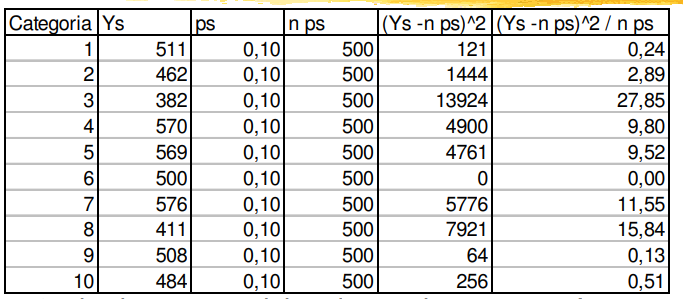
\includegraphics[width=15cm, keepaspectratio]{img/test_chi_quadro.png}
	\caption{Test del Chi-quadro.}\label{fig:chi_quadro}
\end{figure}

\subsection{Test per la verifica delle proprietà di casualità}
I valori $m= 2^31-1$, a=1 e c=1 garantiscono il periodo massimo e l'uniformità di distribuzione dei risultati ma non garantiscono l'assenza di correlazione fra i valori, per rilevare questo problema il test del $X^2$ può essere applicato a coppie di valori estratti dalla sequenza. Nell'esempio di prima si potrebbe dividere il range di valori in 5 sotto-range e formare 25 categorie corrispondenti a tutte le possibili coppie di sotto-range e la $p_s$ si calcola come prodotto delle probabilità di generare un valore in ciascuno di essi. Altri test sono quello del \textbf{gap} ovvero si calcola la lunghezza di sequenze i cui valori sono compresi tra $\alpha$ e $\beta$ e si confronta la loro distribuzione con quella teorica usando il chi-quadro.

\section{Generazione di distribuzioni qualsiasi}
Per la generazione di diverse distribuzioni si utilizzano i seguenti metodi:
\begin{itemize}
    \item\textbf{ Metodo della trasformazione inversa}
    \item \textbf{Metodo del rifiuto}
    \item \textbf{Metodo della composizione}
\end{itemize}

\subsection{Metodo della trasformazione inversa}
\begin{figure}[H]
	\centering
    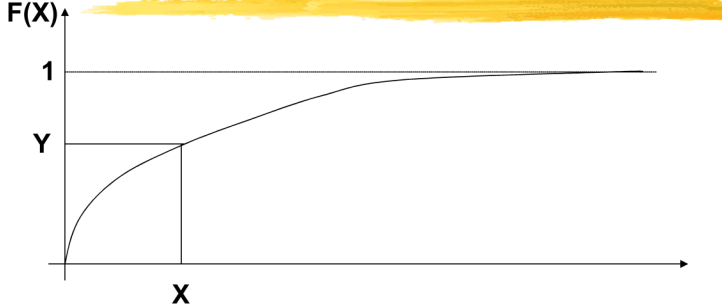
\includegraphics[width=15cm, keepaspectratio]{img/trasformazione_inversa.png}
	\caption{Trasformazione inversa.}\label{fig:trasformazione_inversa}
\end{figure}
Un esempio di applicazione del metodo è la generazione di variabili
casuali distribuite secondo una esponenziale negativa:
\begin{align*}
    & F(x) = 1 - e^{-\mu x} \\
    & 1-y = e^{- \mu x} \\
    & ln(1-y) = ln(e^{-\mu x}) = -\mu x\\
    & x = \dfrac{- ln(1-y)}{\mu}\\ 
\end{align*}
Se y è distribuita come U(0,1), anche Z = 1-Y ha la stessa distribuzione: quindi si può generare una sequenza distribuita secondo una esponenziale negativa semplicemente generando una sequenza con distribuzione U(0,1), applicando la funzione logaritmo naturale, cambiando di segno e dividendo per µ i numeri di tale sequenza.

\subsection{Metodo del rifiuto}
Quando non è facilmente ricavabile l'inversa della cumulativa si utilizzano altri metodi come il metodo del rifiuto.
\begin{figure}[H]
	\centering
    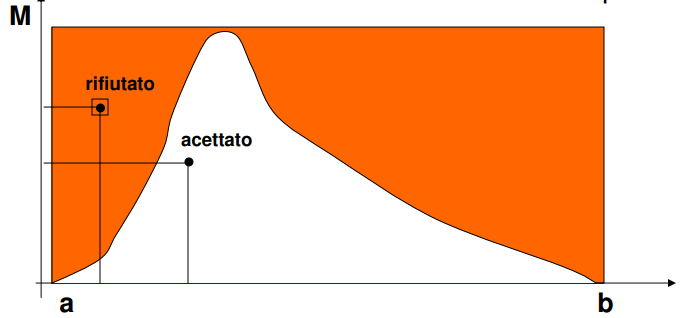
\includegraphics[width=15cm, keepaspectratio]{img/metodo_rifiuto.png}
	\caption{Metodo del rifiuto.}\label{fig:metodo_rifiuto}
\end{figure}
Si genera un valore y distribuito come U(0,M) e un x uniformemente distribuito tra a e b, se $y \leq f(x)$ allora si accetta x come valore generato della distribuzione, sennò si ripete con altri due valori di x e y.

\subsection{Metodo della composizione}
Questa distribuzione può essere vista come risultato della composizione di 4 uniformi: $U(a_1,a_2), U(a_2,a_3), U(a_3,a_4), U(a_4,a_5)$.
\begin{figure}[H]
	\centering
    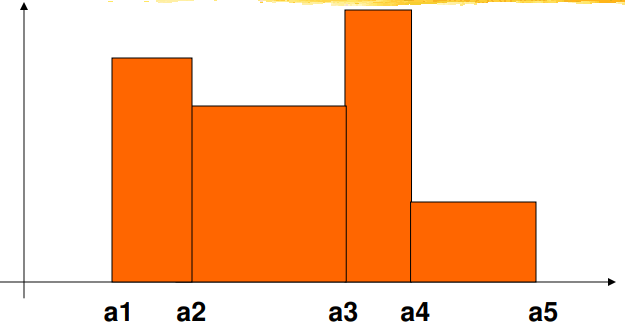
\includegraphics[width=15cm, keepaspectratio]{img/metodo_composizione.png}
	\caption{Metodo della composizione.}\label{fig:metodo_composizione}
\end{figure}
Siano $p_1, p_2, p_3$ e $p_4$ le aree dei quattro rettangoli: per generare un valore tratto da questa distribuzione scegliamo un rettangolo utilizzando le $p_i$, poi generiamo un numero uniformemente distribuito in $U(a_i, a_{i+1})$.

\section{Distribuzioni}
    \newpage
    \chapter{Problemi insolubili} \label{ch:capitolo4}
\subsection{La macchina di turing Universale}
\textbf{Teorema}\\
La funzione g : $N^2 \mapsto N$ definita ponendo, per ogni x , y $\in$ $N$
\begin{center}
    g(x,y) = $\phi_x$(y)
\end{center}
è calcolabile secondo turing.\\\\
\textbf{Dimostrazione}
Su un input (x,y) $\in$ $N^2$
\begin{enumerate}
    \item Decodifica le istruzioni di M$_x$
    
    \item Simula M$_x$ sull’input y
    
    \item Se M$_x$ si arresta, restituisci l’output della computazione
\end{enumerate}
\textbf{Definizione}\\
La macchina di Turing $\mu$ che calcola la funzione g si dice Macchina di Turing universale.\\
La macchina di Turing universale ha la capacità di eseguire qualunque algoritmo.\\
Calcolatore all purpose (modello di Von Neumann).
\newpage
\subsection{La diagonalizzazione}
\textbf{Teorema}
L'insieme $R$ non è numerabile.\\\\
\textbf{Dimostrazione}\\
Per assurdo. Se $R$ fosse numerabile, avremmo una tabella infinita con tutti i numeri reali:\\
\begin{figure}[htp]
    \centering
    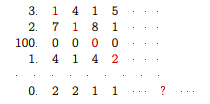
\includegraphics[scale=0.8]{tesi_stile/img/diagonalizzazione.png}
\end{figure}\\
Costruiamo un numero reale x = 0,c$_1$,c$_2$,c$_3$ ... in cui la i-esima cifra decimale è diversa dalla i-esima cifra rossa (e anche da 0 e 9).\\
Per esempio: 0.2211 ...\\
Dove può comparire nella nostra tabella?
\newpage
\subsection{Il problema dell'arresto}
Data una macchina di Turing M e un input y, decidere se M si arresta sull’input y.\\
\begin{center}
    H = \{(x,y) $\in$ $N^2$ $|$ M$_x$ $\downarrow$ y\}
\end{center}
\begin{figure}[htp]
    \centering
    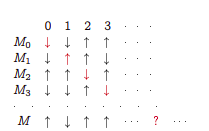
\includegraphics[scale=0.8]{tesi_stile/img/arresto.png}
\end{figure}
Se sapessi risolvere il problema dell’arresto, potrei costruire una macchina di Turing M che su ciascun input x si arresta se e solo se l’elemento x-esimo della diagonale è $\uparrow$.\\
Come prima, tale macchina non può comparire nella nostra tabella!\\
\textbf{Teorema}\\
Il problema dell’arresto non è decidibile.\\\\
\textbf{Dimostrazione}\\
Per assurdo supponiamo che H sia decidibile.\\
Allora anche il problema:
\begin{center}
    K = \{ x $\in$ N $|$ (x , x ) $\in$ H\}
\end{center}
è decidibile.\\
Invero, sia M una macchina di Turing che decide H. Il problema H è deciso dalla macchina M$'$ che esegue il seguente programma:\\
Su input x $\in$ $N$
\begin{center}
    \begin{enumerate}
        \item simula M su (x , x )
        
        \item restituisci l’output della computazione
    \end{enumerate}
\end{center}
\subsection{Il problema dell'arresto2}
Anche il complemento di K è decidibile e, di conseguenza semidecidibile. Più precisamente, K è accettato dalla macchina M$"$ che esegue il seguente programma.\\
Su input x $\in$ $N$
\begin{center}
    \begin{enumerate}
        \item Simula M su (x , x )
        
        \item Se l’output è NO, accetta; se l’output è SI, eseguire un loop infinito
    \end{enumerate}
\end{center}
Sia z l’indice della macchina M$"$. Allora\\
\begin{figure}[htp]
    \centering
    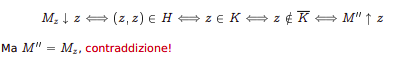
\includegraphics[scale=1]{tesi_stile/img/contraddizione.png}
\end{figure}
\subsection{Riduzioni}
Siano S e T due problemi. Una funzione totale e calcolabile $f$:$N$$\rightarrow$$N$ si dice riduzione del problema S al problema T se, per ogni x $\in$ N si ha:
\begin{center}
    x $\in$ S se e soltanto se $f(x)$ $\in$ T
\end{center}
\textbf{Proposizione}\\
Siano S e T due problemi. Se esite una riduzione di S a T e T è decidibile, allora S è decidibile.\\\\
\textbf{Dimostrazione}\\
Siano M e M$'$ rispettivamente la macchina di Turing che calcola f e quella che decide T. Allora S è deciso dalla macchina che esegue il seguente algoritmo.\\
Su input x
\begin{enumerate}
    \item simula M su x
    
    \item simula M$'$ sull’output di M
    
    \item restituisci l’output di M$'$
\end{enumerate}
\subsection{Riduzioni-2}
\textbf{Corollario}\\
Siano S e T due problemi. Se esite una riduzione di S a T e S è indecidibile, allora anche T è indecidibile.\\\\
\textbf{Proposizione}\\
Siano S e T due problemi. Se esite una riduzione di S a T e T è semidecidibile, allora S è semidecidibile.\\\\
\textbf{Esempio}\\
La funzione x $\in$ $N \mapsto (x,x)$ $\in$ $N^2$ è una riduzione del problema K al problema dell’arresto H.\\\\
\textbf{Osservazione}\\
Il problema dell’arresto è semi-decidibile.\\
Invero, è accettato dalla macchina di Turing universale.\\
\begin{center}
    Il problema\{(x,y, z) $\in$ $N^3$ $|$ M$_x$ $\downarrow$ y in al più z passi\}  \textbf{è decidibile}
\end{center}
\textbf{Teoria della programmazione}\\
Non è possibile costruire un sistema di debugging in grado di stabilire se un
programma termini o meno
\newpage
\subsection{Equivalenza di macchine di Turing}
\textbf{Problema dell’equivalenza di macchine di Turing}\\
Date due macchine di Turing, decidere se calcolano la medesima funzione:
\begin{center}
    E = \{(x , y) $|$ $\phi_x$ = $\phi_y$\}.
\end{center}
\textbf{Osservazione}\\
Due funzioni sono uguali se
\begin{itemize}
    \item hanno lo stesso dominio,
    
    \item hanno lo stesso valore su ogni elemento del dominio.
\end{itemize}
La dimostrazione richiede vari passi che utilizzano diagonalizzazione e riduzione
\newpage
\subsection{Funzioni Totali}
\textbf{Proposizione}\\
Il problema T = \{x $\in$ N $|$ $\phi_x$ è totale\} è indecidibile.\\\\
\textbf{Dimostrazione}\\
Per assurdo, sia T decidibile.\\
Allora c’è una funzione calcolabile totale f tale che T = f($N$).\\
Invero f è calcolata dal seguente algoritmo\\
\begin{figure}[htp]
    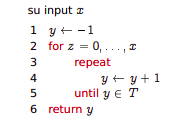
\includegraphics[scale=1]{tesi_stile/img/algo.png}
\end{figure}\\
La funzione g : $N$ $\mapsto$ $N$ definita da
\begin{center}
    g(x) = $\phi_f(x)$ (x)$+$1
\end{center}
è calcolabile totale. Pertanto, g = $\phi_f(z)$ per un opportuno z $\in$ $N$.\\
\begin{figure}[htp]
    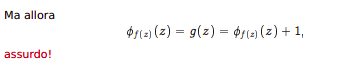
\includegraphics[scale=1]{tesi_stile/img/assurdo.png}
\end{figure}
\newpage
\subsection{Funzione Nulla}
La funzione nulla è la funzione calcolabile totale Z : x $\in$ N $\mapsto$ 0.\\\\
\textbf{Proposizione}\\
Per ogni x $\in$ N, consideriamo la funzione g$_x$ definita da:\\
\begin{figure}[htp]
    \centering
    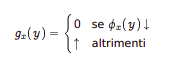
\includegraphics[scale=1]{tesi_stile/img/nulla.png}
\end{figure}\\
Si verifica facilmente che g$_x$ è calcolabile e anche il suo indice è calcolabile.\\
Invero esso è calcolato dal seguente algoritmo:\\
Su input x
\begin{center}
    \begin{enumerate}
        \item calcola il programma di M$_x$
        
        \item aggiungi al programma le istruzioni seguenti:
        \begin{itemize}
            \item se la macchina originale si arresta, output zero
        \end{itemize}
        \item restituisci il codice della macchina modificata
    \end{enumerate}
\end{center}
Quindi g$_x$ = $\phi_h(x)$, con h calcolabile totale. Inoltre\\
\begin{figure}[htp]
    \centering
    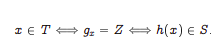
\includegraphics[scale=1]{tesi_stile/img/nulla2.png}
\end{figure}\\
Pertanto h è una riduzione di T a S.\\
Poiché T è indecidibile, lo sarà anche S.
\newpage
\subsection{Equivalenza di macchine di Turing}
\textbf{Proposizione}\\
Il problema E = \{(x , y) $\in$ $N^2$ $|$ $\phi_x$ = $\phi_y$\} è \textbf{indecidibile}\\\\
\textbf{Dimostrazione}\\
Sia z l’indice della funzione nulla.\\
La funzione f : x $\in$ N $\mapsto$ (x,z) $\in$ $N^2$ è una riduzione di S a E.\\
Poiché S è indecidibile, lo sarà anche E.\\\\
\textbf{Osservazione}\\
Non è possibile decidere se due generici programmi calcolano la stessa funzione: la correttezza semantica di un programma è indecidibile.







    \newpage
    \chapter{Modelli a singola coda}
Un modello a cosa è costituito dalla rappresentazione di un sistema di congestione in cui utenti che provengono da una popolazione si mettono in coda per ottenere il servizio richiesto da un insieme di risorse o serventi. Una coda è una linea di attesa per un servizio. L'insieme formato da cosa e serventi è detto \textbf{centro di servizio}. 

\begin{figure}[H]
	\centering
    \includegraphics[width=15cm, keepaspectratio]{img/modello_coda.png}
	\caption{Sistema di congestione.}\label{fig:modello_coda}
\end{figure}
Un sistema a coda è costituito da alcune grandezze che sono:
\begin{itemize}
    \item $\Delta$ tempo di interarrivo;
    \item w numero di utenti in cosa e $t_w$ tempi di attesa in coda, tempo che intercorre fra l'arrivo di un utente e l'istante in cui entra in servizio;
    \item s numero di utenti in coda e $t_s$ tempo di servizio, tempo fra inizio e completamento del servizio;
    \item q numero di utenti nel sistema e $t_q$ tempo di risposta, tempo fra arrivo e partenza dal sistema dello stesso utente.
\end{itemize}
Per definizione $q= w+s$ e le variabili di tempi sono legati dalla seguente relazione $t_q = t_w + t_s$.

Fra queste tipicamente alcune sono parametri del sistema, quali $t_s$ e $\Delta$ mentre le altre sono oggetto di analisi e di valutazione.
\paragraph{Processo di arrivo}
Assumiamo che il tempi di interarrivo $ \Delta$ siano variabili casuali statisticamente indipendenti con la stessa distribuzione di probabilità.
\paragraph{Domanda di servizio, tasso di servizio e tempo di servizio}
La quantità di servizio richiesta da un utente ad un centro di servizio è detta
domanda di servizio ed è espressa in unità di tempo. La velocità o tasso di servizio di un servente è una caratteristica del servente, ovvero della risorsa, ed è espressa in unità di servizio per unità di tempo. Il tempo di servizio è la il rapporto fra la domanda di servizio e la velocità di servizio espresso in unità di tempo.
\paragraph{Disciplina di servizio}
Una \textbf{disciplina di servizio} è un algoritmo di ordinamento degli utenti in coda in base al quale viene selezionato l'utente da servire, ovvero l’ordine con cui estrarre gli utenti dalla coda. Alcuni esempi sono FIFO che serve gli utenti in ordine di arrivo  e LIFO che serve gli utenti in ordine inverso al tempo di
arrivo. La disciplina di servizio RAND determina l’utente da estrarre dalla coda e servire
in modo casuale, secondo la distribuzione unforme discreta. Le \textbf{discipline a priorità} determinano l’ordine di servizio degli utenti sulla base di priorità assegnate ad esse. La disciplina round robin è un esempio di disciplina che dipende dalla quantità di servizio già assegnato. Tale algoritmo assegna il servente ciclicamente agli utenti per un intervallo massimo di tempo detto quanto.

\subsection{Notazione di Kendall} Per descrivere e definire i modelli a coda singola Kendall
ha introdotto la seguente notazione:
\[ A/B/c/n/p/Z\]
dove i simboli denotano:
\begin{itemize}
    \item A : distribuzione del tempo di interarrivo;
    \item B : distribuzione del tempo di servizio $t_s$;
    \item c : numero di serventi m;
    \item n : dimensione della coda ovvero la capacità del centro, q;
    \item p : dimensione della popolazione;
    \item  Z : disciplina di servizio.
\end{itemize}
 Tale notazione si semplifica in A/B/c quando coda e popolazione sono illimitate e
la disciplina di servizio è FIFO, ovvero se $n=p=\infty$ e Z=FIFO. D denota la distribuzione deterministica o costante, M la distribuzione esponenziale negativa,$H_h$ l’iperesponenziale ad h stadi,$E_k$ l’Erlangiana a k stadi e G la generale.
Il comportamento del sistema nel tempo può essere analizzato in un tempo finito.
In tal caso si parla di \textbf{analisi transiente}. Quando il sistema raggiunge le condizioni di
equilibrio in un tempo che tende ad infinito, ovvero se il sistema è stabile si effettua
\textbf{l’analisi stazionaria.} Tale analisi porta alla valutazione degli indici di prestazione del sistema di code, in particolare di:
\begin{itemize}
    \item numero di utenti nel sistema q;
    \item numero di utenti in coda w;
    \item tempo di risposta $t_q$;
    \item tempo di attesa $t_w$;
    \item utilizzazione U;
    \item throughput X.
\end{itemize}
Le prime quattro sono variabili casuali di cui si valuta la distribuzione di probabilità,
e/o i momenti. Possiamo scrivere immediatamente le seguenti
relazioni fra i valori medi:

\begin{align}
    & E[q] = E[w] + E[s]\\
    & E[t_q] = E[t_w] + E[t_s]
\end{align}

Una relazione fondamentale nella teoria delle code è rappresentato dal \textbf{teorema di
Little} il quale stabilisce che il numero medio di utenti in un sistema è uguale al
prodotto fra il throughput e il tempo medio di risposta, ovvero:

\begin{align}
   & E[q] = X E[t_q] \\
   & E[w] = X E[t_w]
\end{align}

\subsection{Modelli basilari di code: i sistemi M/M/1 ed M/M/m}
M/M/1 costituisce la base per la definizione di modelli più
complessi a struttura reticolare e per lo sviluppo gerarchico di modelli a diversi livelli
di astrazione. Nella notazione di Kendall il sistema di code M/M/1 denota un sistema aperto
formato da un singolo centro di servizio con:
\begin{itemize}
    \item distribuzione del tempo di interarrivo esponenziale, di parametro $\lambda$,
    \item tempo di servizio degli utenti indipendente e con identica distribuzione
esponenziale di parametro $\mu$,
    \item singolo servente.
\end{itemize}
La disciplina di servizio è FIFO e sia la memoria che la popolazione sono infinite.
\begin{figure}[H]
	\centering
    \includegraphics[width=13cm, keepaspectratio]{img/sistema_mm1.png}
	\caption{Sistema M/M/1.}\label{fig:mm1}
\end{figure}

Per le ipotesi di esponenzialità dei tempi di interarrivo e di servizio, gli unici eventi possibili che si osservano in un intervallo di tempo $d_t$ quando nel sistema vi sono k utenti sono i seguenti:
\begin{enumerate}
    \item nessun arrivo e nessun completamento di servizio (permanenza nello stato k);
    \item un arrivo e nessun completamento di servizio (transizione dallo stato k allo stato k+1
con probabilità $\lambda dt$);
    \item nessun arrivo e un completamento di servizio (transizione dallo stato k allo stato k-1
con probabilità $\mu dt$);
    \item uno o più arrivi e uno o più completamenti di servizio (transizione con probabilità
trascurabile rispetto alle altre transizioni per l’ipotesi di esponenzialità).
\end{enumerate}

\subsection{Analisi stazionaria}
Definiamo l’intensità di traffico del sistema come rapporto fra tempo medio di servizio e tempo medio di interarrivo, denotato da $\rho = \lambda / \mu$. La condizione di
stazionarietà del sistema M/M/1 richiede che $\rho <1$, ovvero che il tasso di arrivo al
sistema sia minore del tasso di servizio, $\lambda < \mu$. La distribuzione di probabilità di stato in
equilibrio  si ricava :
\begin{align}
    & \pi_0 = 1- \rho \\
    &\pi_k = \rho^k \pi_0 = \rho (1-\rho) & k>0
\end{align}
la distribuzione di probabilità del numero di utenti nel sistema in condizioni stazionarie è geometrica a ragione $\rho$. \\
Il numero medio di utenti nel sistema, che denotiamo con N=E[q], si può immediatamente ricavare come:
\begin{align}
    N = \frac{\rho }{1-\rho} 
\end{align}
e la varianza del numero di utenti, denotata da Var[q], è
\begin{align}
    Var[q] = \frac{\rho}{(1-\rho)^2}
\end{align}
Per la relazione (5.1) ricaviamo immediatamente il numero medio di utenti in coda,
denotato da W=E[w], poiché $E[s] =\rho$ ed E[q]=N:
\begin{align}
    W = N-\rho = \frac{\rho^2 }{1-\rho}
\end{align}

Il tempo medio di risposta, denotato da R=E[tq], si ricava dal teorema di Little  che per il sistema M/M/1 assume la forma $N= \lambda R$:
\begin{align}
    R = \frac{\frac{1}{\mu}}{1-\rho}
\end{align}

Infine il tempo medio di attesa in coda,$T_w=E[t_w]$ si ottiene o dal teorema di Little come $W = \lambda T_w$ o dalla relazione (3.4) ovvero $R = T_w +T_s$, dove $T_s = \frac{1}{\mu}$ denota il tempo medio di servizio, da cui si ricava
\begin{align}
    T_w = \frac{\frac{\rho}{\mu}}{1-\rho}
\end{align}

L’utilizzazione è esprimibile per il sistema M/M/1 come:
\begin{align}
    U = 1 -\pi_0 = \rho
\end{align}

Dalla distribuzione di probabilità (5.6) possiamo calcolare la probabilità con cui si
osservano almeno k utenti nel sistema in condizioni di equilibrio:
\begin{align}
    & Prob \{ \textrm{numero di utenti nel sistema $\geq$ k}\}= \sum_{i\geq k}^{} \pi_i= (1-\rho) \sum_{i\geq k}^{} \rho_i =\rho^k
\end{align}

\subsection{Sistema M/M/$\infty$ : serventi infiniti}
Un modello M/M/$\infty$ permette di rappresentare un sistema nel quale ad ogni
arrivo vi è sempre un servente libero.In un sistema di questo tipo non si forma quindi
mai coda, poiché ogni utente riceve immediatamente servizio dall’istante in cui arriva
al sistema. Il processo stocastico {q(t) | t>0} associato al sistema $M/M/\infty$ è un processo di
nascita e morte con tassi di nascita $\lambda_k=\lambda, k\geq0, $e con tassi di morte $\mu_k= k \mu, k\geq1$. La condizione di stazionarietà è certamente sempre soddisfatta quindi il
sistema è sempre stabile. esiste la distribuzione stazionaria del numero di utenti nel
sistema, che coincide con il numero di serventi occupati da cui si ricava:
\begin{align}
    & \pi_k = \frac{\rho^k}{k!} e^{-\rho} & k\geq 0
\end{align}
dove $\rho = \lambda/\mu$.
Si ricava immediatamente il numero medio di utenti nel sistema 
\begin{align}
    N = \rho
\end{align}
Dato che nel sistema $M/M/\infty $ gli utenti non sperimentano mai coda, il tempo medio
di risposta coincide con il tempo medio di servizio:
\begin{align}
    R = T_s = \frac{1}{\mu}
\end{align}

\subsection{Sistema M/M/m: serventi multipli}
Il sistema aperto M/M/m è caratterizzato da un processo di arrivo Poissoniano di $\lambda$
parametro, distribuzione del tempo di servizio esponenziale di parametro $\mu$ e un
numero di serventi m>0. Come in M/M/1  il tasso medio di servizio dipende dallo stato k secondo la seguente funzione $\mu(k) = k \mu$ ,$0\leq k\leq m, e \mu(k) = m \mu, k>m$.  Definiamo l’intensità di traffico come $\rho =\lambda/ m\mu$. In questo caso esiste la distribuzione stazionaria del numero di utenti nel sistema :
\begin{align}
    & \pi_k = \frac{(m\rho)^k}{k!}\pi_0 & 0\leq k \leq m \\
    &\pi_k = \frac{m^m \rho^k}{m!}\pi_0 & k>m \\
    &\pi_0 = \left [  \sum_{k=0}^{m-1} \frac{(m\rho)^k}{k!} +  \frac{(m\rho)^m}{m!}\cdot \frac{1}{1-\rho} \right ]^{-1}
\end{align}
Il numero medio di serventi occupati E[s] è dato da
\begin{align}
    & E[s] = \sum_{k=0}^{m-1} k \pi_k + \frac{m\pi_m}{1-\rho} = m\rho = \frac{\lambda}{\mu}
\end{align}
dove $\rho$ rappresenta l’utilizzazione di ogni singolo servente.
Il numero medio di utenti nel sistema è dato da
\begin{align}
    & N = m \rho + \pi_m \frac{\rho}{(1-\rho)^2} \\
    & W = \pi_m \frac{\rho}{(1-\rho)^2}
\end{align}
Il tempo medio di risposta si ottiene applicando il teorema di Little $N=\lambda R$ ottenendo:
\begin{align}
    R = \frac{1}{\mu} + \frac{\pi_m}{(m\mu(1-\rho)^2)}
\end{align}

Similmente, otteniamo il tempo medio di attesa:
\begin{align}
    T_W = \frac{\pi_m}{m\mu ( 1-\rho)^2}
\end{align}
La probabilità che un utente in arrivo trovi tutti i serventi occupati e quindi
sperimenti coda è data dalla formula di Erlang-C:
\begin{align}
    Prob\{\textrm{coda}\} = \sum_{k=m}^{\infty}\pi_k = \pi_0 \frac{(m\rho)^m}{!m} \cdot \frac{1}{1-\rho}
\end{align}
Questa formula, è stata applicata per lo studio di sistemi di traffico telefonico per valutare la probabilità che una chiamata (un utente) trovi tutti i canali di comunicazione (i serventi) occupati.
\\
Vedere esercizio \ref{es:m/m/m}.

\subsection{Sistema M/M/1/K : memoria finita}
Consideriamo il sistema M/M/1 nel quale sono ammessi al più K utenti. Il processo di arrivo è Poissoniano di parametro $\lambda$, ma un utente che arrivando trova il sistema completo, cioè con K utenti già presenti, non viene accettato e viene perso. Il processo stocastico ${q(t) | t>0}$ associato al sistema M/M/1/k è un processo di nascita e morte con spazio degli stati finito $E=\{0,1,\cdots, K\}$ e tassi di nascita $\lambda_k=\lambda$,$ 0 \leq k<K$, e tassi di morte $\mu_k= \mu$, $1\leq k<K-1$ e $\lambda_k=0$ e $\mu_k= 0$ altrove. La condizione di stazionarietà è certamente verificata, poiché il processo è finito e irriducibile e quindi ergodico. La distribuzione stazionaria del numero di utenti nel sistema
definita dalle formule:
\begin{align}
    & \pi_k = \frac{1-\rho}{1 -\rho^{K+1}} \rho & 0\leq k \leq K \\
    & \pi_k = 0 & k>K
\end{align}
Nel caso particolare di K=1 lo spazio è formato da due soli stati e si ricava
\begin{align}
    & \pi_0 = \frac{\mu}{\lambda +\mu}\\
    & \pi_1 = \frac{\lambda}{\lambda + \mu}
\end{align}

\subsection{Sistema M/M/1//M: popolazione finita}
Consideriamo il sistema M/M/1 assumendo che gli utenti provengano da una popolazione finita, di dimensione M>0.
    \newpage
    \chapter{Auto-riferimento} \label{ch:capitolo6}
\section{Autoriferimento}
\subsection{Teorema di ricursione di Turing}
\textbf{Teorema}\\
Sia $f: N $ x $N \mapsto N$ una funzione calcolabile (parziale). Esiste effettivamente $z \in N$ tale che:
\begin{center}
    $\phi_z (y) = f(z,y).$
\end{center}
\textbf{Osservazione}
\begin{itemize}
    \item Il programma di una macchina di Turing può accedere al suo codice
    
    \item Si può calcolare una funzione che dipende anche dalla macchina che la calcola
\end{itemize}
\textbf{Esempio}\\
Cosa calcola la seguente macchina di Turing?.\\
Su input x
\begin{figure}[htp]
    \includegraphics[scale=0.8]{tesi_stile/img/cap6f1.png}
\end{figure}
\subsection{Teorema s-m-n}
\textbf{Teorema}\\
Sia $f : N $ x $N \mapsto N$ una funzione (parziale) calcolabile. Allora esiste una funzione calcolabile totale $t:N \mapsto N$ tale che
\begin{center}
    $\phi_{t(x)} (y)=f(x,y)$ con $x,y \in N.$
\end{center}
\textbf{Osservazione}\\
Questo teorema ci dice che ogni funzione di due variabili f(x,y) si può calcolare nel modo seguente:
\begin{itemize}
    \item costruisco una macchina di Turing $M = M_t(x)$ che dipende solo da x
    
    \item eseguo M sull'input y
\end{itemize}
\newpage
\subsection{Dimostrazione del Teorema s-m-n}
\textbf{Dimostrazione}\\
Per ogni $x \in N,$ sia $g_x: N \mapsto N$ la funzione definita da $g_x(y) = f(x,y)$.\\\\
Una macchina di Turing per calcolare gx si ottiene concatenando
\begin{itemize}
    \item le istruzioni per stampare x sul nastro prima di y
    
    \item le istruzioni della macchina di Turing che calcola f .
\end{itemize}
Dato x, si può effettivamente costruire tale macchina e calcolarne l’indice.\\
Se t è la funzione che esegue questo calcolo, si avrà\\
\begin{center}
    $f(x,y)=g_x(y) = \phi_{t(x)}(y).$\\
\end{center}
\begin{figure}[htp]
    \centering
    \includegraphics[scale=0.8]{tesi_stile/img/cap6foto2.png}
\end{figure}
\newpage
\subsection{Dimostrazione del Teorema di Ricursione}
Per ogni $x \in N$, sia $g_x : N \mapsto N$ la funzione definita da $g_x(y) = f(x,y)$.
\begin{figure}[htp]
    \centering
    \includegraphics[scale=0.9]{tesi_stile/img/cap6f3.png}
\end{figure}
\\Una macchina di Turing per calcolare $g_x$ si ottiene concatenando.\\
Per il Teorema s-m-n, c’è una funzione totale t = $\phi_v$ tale che\\
\begin{center}
    $\phi_{t(z)}(y) = g(x,y)$ con $x,y \in N$
\end{center}
Posto $z = t(v) = \phi_v (v)$, si ha
\begin{center}
   $ \phi_z(y) = \phi_t{(v)}(y) = g(v,y)=f(\phi_v(v), y) = f (z,y)$
\end{center}
\newpage
\subsection{Costruzione}
\begin{figure}[htp]
    \centering
    \includegraphics[scale=1]{tesi_stile/img/cap6f4.png}
\end{figure}
\newpage
\subsection{Esempio}
È indecidibile se una macchina di Turing accetta 1.\\
Se così non fosse, potremmo costruire una macchina di Turing con il seguente programma\\
Su input x.\\
\begin{figure}[htp]
    \includegraphics[scale=0.8]{tesi_stile/img/cap6f5.png}
\end{figure}\\
\begin{center}
    \textbf{Contraddizione!}
\end{center}
Nuova dimostrazione dell’indecidibilità del problema dell’arresto:\\
Se fosse decidibile, potremmo costruire una macchina di Turing con il seguente programma.\\
Su input x.\\
\begin{figure}[htp]
    \includegraphics[scale=0.8]{tesi_stile/img/cap6f6.png}
\end{figure}\\
\begin{center}
    \textbf{Contraddizione!}
\end{center}
\newpage
\subsection{Teorema del punto fisso}
\textbf{Teorema}\\
 Sia $t : N \mapsto N$ una funzione calcolabile totale.\\
 Esiste effettivamente $z \in N$ tale che\\
 \begin{center}
     $\phi_z = \phi_t(z)$
 \end{center}
 \textbf{Dimostrazione}\\
La funzione $f : N$ x $N \mapsto N$ definita da $f(x,y) = \phi_{t(x)}(y)$ con $x,y \in N$, è
calcolabile. Per il Teorema di Recursione ci sarà $z \in N$ tale che\\
\begin{center}
    $\phi_z (y) = f (z,y) = \phi_t(z) (y),  y \in N.$
\end{center}
\textbf{Oppure}\\
Basta considerare la funzione calcolata dalla procedura.\\
Su input x\\
\begin{figure}[htp]
    \includegraphics[scale=0.8]{tesi_stile/img/cap6f7.png}
\end{figure}
\newpage
\subsection{Teorema di Radice}
\textbf{Teorema}\\
Sia P una famiglia di funzioni calcolabili. L’insieme.\\
\begin{center}
    $R = \{x \in N | \phi_x \in P\}$
\end{center}
è indecidibile, purchè $R\neq \varnothing$, $N$.\\\\
\textbf{Dimostrazione}\\
Per assurdo, supponiamo che R sia decidibile e $R \neq \varnothing$, $N$. 
\begin{itemize}
    \item Possiamo trovare $i \in R$ e $j \notin R$.
    
    \item Definiamo la funzione $f : N $ x $N \mapsto N$ con
\end{itemize}
\begin{figure}[htp]
    \centering
    \includegraphics[scale=0.8]{tesi_stile/img/cap6f8.png}
\end{figure}
Per il Teorema di Recursione ci sarà $z \in N$ tale che $\phi_z (y) = f(z,y)$.\\
Ma allora se $z \notin R$, si ha $\phi_z = \phi_i \in R$, mentre se $z \in R$, si ha $\phi_z = \phi_j \notin R$.\\
\begin{center}
    \centering
    \textbf{Contraddizione!}.
\end{center}
\newpage
\subsection{Macchina di Turing minimali}
\textbf{Definizione}\\
Una macchina di Turing è minimale se non esistono macchine di Turing con un minor numero di stati che calcolano la stessa funzione.\\\\
\textbf{Osservazione}\\
Legata alle nozioni di complessità di Kolmogorov, entropia, compressibilità.\\\\
\textbf{Proposizione}\\
È indecidibile se una macchina di Turing è minimale.\\\\
\textbf{Dimostrazione}\\
Se così non fosse, avremmo una macchina di Turing che:\\
Su input x
\begin{figure}[htp]
    \includegraphics[scale=0.8]{tesi_stile/img/cap6f9.png}
\end{figure}
\\Ma allora Mz è equivalente a una macchina minimale con più stati: \textbf{assurdo}
    \newpage
    
\chapter{Esercizi}

\section{Esercizio su M/M/m} \label{es:m/m/m}
La clinica oculistica dell’Ospedale offre ogni mercoledì pomeriggio dei test gratuiti della vista.
Ci sono 3 oculisti in contemporanea. Un test impiega, in media, 20 minuti e il tempo reale è stato
riscontrato essere approssimativamente distribuito in modo esponenziale intorno a questa media.
I clienti arrivano in accordo ad un processo di Poisson con un tasso medio di 6 all’ora e i pazienti
sono serviti seguendo una politica FIFO.\\

\noindent I dirigenti dell’Ospedale sono interessati a conoscere:
\begin{enumerate}
    \item Quale è il numero medio di persone in attesa?
    \item Quale è il tempo medio speso da un paziente nella clinica?
    \item Quale è la percentuale media del tempo in cui i dottori non lavorano?
    \item Quale è la frazione di tempo nella quale un cliente che arriva trova almeno 1 dottore libero.
\end{enumerate}

\subsection{Soluzione}
Troviamo alcuni parametri, m=3 $\mu= \frac{1}{20}/min = \frac{20}{60} = \frac{1}{3}/ora$ questo vuol dire che in un ora vengono effettuate 3 visite, $\lambda = 6/ora$ quindi
\[\rho = \frac{\lambda}{\mu m} = \frac{6}{3 \cdot 3} = \frac{2}{3} < 1 \]

\begin{enumerate}
    \item  Il numero medio di persone in attesa è
            \begin{align*}
                 & W = \pi_m \frac{\rho}{(1-\rho)^2} = \frac{4}{27} \cdot \frac{2/3}{(1-2/3)^2} = \frac{8}{9}\\
                 & \pi_0 = \left [  \sum_{k=0}^{m-1} \frac{(m\rho)^k}{k!} +  \frac{(m\rho)^m}{m!}\cdot \frac{1}{1-\rho} \right ]^{-1} = \left [  \sum_{k=0}^{2} \frac{(3 \cdot 2/3)^k}{k!} +  \frac{(3 \cdot 2/3)^3}{3!}\cdot \frac{1}{1-2/3} \right ]^{-1} = \\
                 & \left [ \frac{2^0}{0!}+ \frac{2^1}{1!} + \frac{2^2}{2!} + 4 \right]^{-1} = [9]^{-1} = \frac{1}{9}\\
                 & \pi_k = \frac{(3\cdot 2/3)^3}{3!} \frac{1}{9} = \frac{8}{54} = \frac{4}{27}
            \end{align*}
    
    \item Il tempo medio speso da un paziente nella clinica è:
            \begin{align*}
                   & R = \frac{1}{\mu} + \frac{\pi_m}{(m\mu(1-\rho)^2)} = \frac{1}{\frac{1}{20}} + \frac{}{}\pi_m
            \end{align*}
\end{enumerate}


    \newpage
    % ...
    \bibliographystyle{plainnat}
    % Opzionale
    \newpage
    % \bibliography{bibliografia}
	

    
\end{document}
